\chapter{Pattern Matching for Phrases with Gaps}\label{chap:algorithms}

\begin{quote}
	{\em People who analyze algorithms have double happiness. First of all they experience the sheer beauty of elegant mathematical patterns that surround elegant computational procedures. Then they receive a practical payoff when their theories make it possible to get other jobs done more quickly and more economically.}  
	\begin{flushright}
		--Donald Knuth
	\end{flushright}
\end{quote}

Phrase-based translation is an important milestone in
statistical machine translation, but as we saw in Chapter~\ref{chap:survey},
it is far from the final word in translation modeling.  In the last few
years, statistical MT models have greatly diversified.
Most new models are inspired in some way by phrase-based translation, and motivated by
a desire to overcome its weaknesses.  Some notable examples include non-contiguous
phrase-based models \citep{Simard:2005:hlt-emnlp}, hierarchical phrase-based
models \citep[\textsection\ref{sec:hiero}]{Chiang:2005:acl,Chiang:2007:cl}, dependency treelet models
\citep{Quirk:2005:acl,Quirk:2006:hlt-naacl}, and syntax-based tree-to-string
transducer models \citep{Galley:2004:naacl,Galley:2006:acl,DeNeefe:2007:emnlp-conll}.

Given the heterogeneity of these models, it is notable that they all share
three specific characteristics.  First, like phrase-based models,
they can translate multi-word units.  Second, unlike phrase-based models,
they can also translate phrases with gaps---that is, multi-word
units composed of words that are not contiguous in the source sentence.
Finally, as a consequence of their greater expressivity, they
all require many more rules than standard phrase-based models.  In general,
the ruleset extracted from a corpus by any of them
is at least an order of magnitude larger than the ruleset of a phrase-based
model extracted from the same data.  In fact, the vast size of extracted
rulesets is a recurring topic in the literature of these models
\citep[see, e.g.][]{Chiang:2007:cl,DeNeefe:2007:emnlp-conll,Simard:2005:hlt-emnlp}.

The size of these rulesets makes efficient scaling techniques even 
more relevant to these models than it was to standard phrase-based models.
However, the introduction of gaps
poses an algorithmic challenge for translation by pattern matching.  The
pattern matching algorithm presented in Chapter~\ref{chap:overview} depended 
crucially on the fact that our query pattern was a contiguous string.  
If we no longer enforce contiguity, we
require new algorithms for pattern matching.  To the extent that phrases 
with gaps represent the future of statistical machine translation, the 
relevance of translation by pattern matching depends on its applicability
to these models.  We therefore seek to develop efficient pattern matching
algorithms for models where source phrases contain gaps.

To make matters concrete, we will focus on hierarchical phrase-based
translation \citep[\textsection\ref{sec:hiero}]{Chiang:2005:acl,Chiang:2007:cl}.  This model gives
statistically significant improvements in BLEU score over a standard 
phrase-based system trained on the same data.  Although we 
consider this specific model, we emphasize
that our pattern matching algorithms are general enough to be
applied to any of the aforementioned models, with the proviso that the
source-driven rule extraction algorithm is model-specific and must
be redeveloped for each case.

With this mind, we can now succinctly state the problem of this
chapter: {\em Given an input sentence, efficiently find and extract
all hierarchical phrase-based translation rules for that 
sentence in the training corpus.}

We first review the relevant aspects of 
hierarchical phrase-based translation
(\textsection\ref{sec:hierarchical-translation}).  
We show that the obvious solution using 
state-of-the-art pattern matching algorithms is 
hopelessly inefficient (\textsection\ref{sec:problem}).  We then describe a series 
of algorithms to address this inefficiency (\textsection\ref{sec:solution}).
Our algorithms reduce computation time by two orders of magnitude, making
the approach feasible and enabling us to replicate state-of-the-art
translation accuracy (\textsection\ref{sec:hiero-results}).


\section{Hierarchical Phrase-Based Translation (Redux)}\label{sec:hierarchical-translation}

\setlength{\fboxsep}{1pt}
\newcommand{\nt}[2]{#1_{\framebox{\scriptsize #2}}}

Hierarchical phrase-based 
translation is based on synchronous context-free grammar
(\textsection\ref{sec:hiero}).  The lexicalized translation rules of
this grammar may contain a single nonterminal symbol, denoted $X$.  
We will use $a$, $b$, $c$ and $d$ to denote terminal symbols, and $u$,
$v$, and $w$ to denote (possibly empty) sequences of these terminals.
We will additionally use $\alpha$ and $\beta$ to denote
(possibly empty) sequences containing both terminals and nonterminals.
A translation rule is written $X \rightarrow \alpha / \beta$.
This rule states that a span of the input matching $\alpha$ is replaced
by $\beta$ in translation.  We require that $\alpha$ and $\beta$ contain
an equal number (possibly zero) of coindexed nonterminals.  
An example rule with coindexes is
$X \rightarrow u\nt{X}{1}v\nt{X}{2}w / u'\nt{X}{2}v'\nt{X}{1}w'$.  When
discussing only the source side of such rules, we will leave out
the coindexes.  For instance, the source side of the above rule will be written
$uXvXw$.\footnote{In the canonical representation of the grammar,
source-side coindexes always appear in numerical order, so source phrases
are unambiguous despite this simplification.}

The pattern matching problem for this model is illustrated in 
Figure~\ref{fig:hiero-query} (cf. Figure~\ref{fig:pb-query}).  
If arbitrary sequences of terminals
and nonterminals may be rules, then the number of source phrases
that cover a sentence is exponential in sentence length.  This is
especially problematic for training the model.  \citet{Chiang:2007:cl}
employs several heuristics to limit the size of the extracted grammar.

\figpreamble
\begin{figure}
	\figfontsize{
	\begin{center}
		\noindent Input Sentence:
{\em it persuades him and it disheartens him}

~

\noindent Query Patterns:
{\em
it, persuades, him, and, disheartens, 
it~persuades, persuades~him, him~and, and~it, it~disheartens, disheartens~him,
it~persuades~him, persuades~him~and, him~and~it, and~it~disheartens, it~disheartens~him,
it~persuades~him~and, persuades~him~and~it, him~and~it~disheartens, and~it~disheartens~him,
it~persuades~him~and~it, persuades~him~and~it~disheartens, him~and~it~disheartens~him,
it~persuades~him~and~it~disheartens, persuades~him~and~it~disheartens~him,
it~persuades~him~and~it~disheartens~him,
% 2 words + 1 nonterminal
it~X~him, it~X~and, it~X~it, it~X~disheartens, it~X~him,
persuades~X~and, persuades~X~it, persuades~X~disheartens, persuades~X~him,
him~X~it, him~X~disheartens, him~X~him,
and~X~disheartens, and~X~him,
% 3 words + nonterminals
it~X~him~and, it~X~and~it, it~X~it~disheartens, it~X~disheartens~him,
it~persuades~X~and, it~persuades~X~it, it~persuades~X~disheartens, it~persuades~X~him,
it~X~him~X~it, it~X~him~X~disheartens, it~X~him~X~him,
it~X~and~X~disheartens, it~X~and~X~him,
it~X~it~X~him,
persuades~X~and~it, persuades~X~it~disheartens, persuades~X~disheartens~him,
persuades~him~X~it, persuades~him~X~disheartens, persuades~him~X~him,
persuades~X~and~X~disheartens, persuades~X~and~him,
persuades~X~it~X~him,
him~X~it~disheartens, him~X~disheartens~him, 
him~and~X~disheartens, him~and~X~him,
him~X~it~X~him,
% 4 words + nonterminals
it~X~him~and~it, it~X~and~it~disheartens, it~X~it~disheartens~him, 
it~persuades~X~it~disheartens, it~persuades~X~disheartens~him,
it~persuades~him~X~disheartens, it~persuades~him~X~him,
it~X~him~X~it~disheartens, it~X~him~X~disheartens~him,
it~X~him~and~X~disheartens, it~X~him~and~X~him,
it~X~and~it~X~him,
it~persuades~X~and~X~disheartens, it~persuades~X~and~X~him,
it~persuades~X~it~X~him,
it~X~him~X~it~X~him,
persuades~X~and~it~disheartens, persuades~X~it~disheartens~him,
persuades~him~X~it~disheartens, persuades~him~X~disheartens~him, 
persuades~him~and~X~disheartens, persuades~him~and~X~him,
him~X~it~disheartens~him,
him~and~X~disheartens~him,
him~and~it~X~him,
% 5 words + nonterminals
it~X~him~and~it~disheartens,
it~X~and~it~disheartens~him,
it~persuades~X~and~it~disheartens,
it~persuades~X~it~disheartens~him,
it~persuades~him~X~it~disheartens,
it~persuades~him~X~disheartens~him,
it~persuades~him~and~X~disheartens,
it~persuades~him~and~X~him,
it~X~him~X~it~disheartens~him,
it~X~him~and~X~disheartens~him,
it~X~him~and~it~X~him,
it~persuades~X~and~X~disheartens~him,
it~persuades~X~and~it~X~him,
it~persuades~him~X~it~X~him,
persuades~X~and~it~disheartens~him,
persuades~him~X~it~disheartens~him,
persuades~him~and~X~disheartens~him,
persuades~him~and~it~X~him,
% 6 words + nonterminals
it~X~him~and~it~disheartens~him,
it~persuades~X~and~it~disheartens~him,
it~persuades~him~X~it~disheartens~him,
it~persuades~him~and~X~disheartens~him,
it~persuades~him~and~it~X~him,
}.

	\end{center}}
	\figpostamble
\caption[Example input sentence and resulting query pattern for hierarchical phrase-based translation.]{Example input sentence and resulting query 
patterns for hierarchical phrase-based translation.  There
are many more query patterns than for a standard phrase-based system
on the same sentence (cf. Figure~\ref{fig:pb-query}).}
\label{fig:hiero-query}
\end{figure}

\begin{itemize}
	\item The span of any extracted rule in either the source or target text is restricted to some small value (henceforth $\maxphrasespan$).
	\item The number of nonterminal symbols in a rule is restricted to some small value (henceforth $\maxnts$).
	\item The total number of terminal and nonterminal symbols in the source side of a rule is restricted to some small value (henceforth $\maxphraselen$).\footnote{\citet{Chiang:2007:cl} does not explicitly restrict the number of target-side symbols, making $\maxphrasespan$ the {\em de facto} limit.}
%	\item Nonterminals are required to have a {\em minimum} span in the training data (henceforth $\mingapsize$).  If the span is one word, then nearly every word could be subtracted to form a nonterminal.  Therefore we can decrease the grammar size by increasing the minimum span.
\end{itemize}

\noindent Our algorithms are parameterized for these constraints
so they don't depend in any way on specific values for them.  We explore
this in greater detail in Chapter~\ref{chap:scaling}.

Abstractly, translation by pattern matching can be applied
using the same generic algorithm that we used for the standard
phrase-based model.

\begin{enumerate}
	\item Enumerate all source phrases that are licensed by the model.
	\item Query the source training text for each source phrase.
	\item Extract and score the translations of each source phrase.
	\item Decode using the scored translation rules.
\end{enumerate}

\noindent Implementing these steps for the hierarchical phrase-based
model requires new algorithms for pattern matching and phrase extraction.

\section{The Pattern Matching Problem for Hierarchical Phrases}\label{sec:problem}

As with standard phrase-based models, we can search for a contiguous source
phrase $\alpha=u$ using a suffix array (\textsection\ref{sec:suffix_arrays}).
However, source phrases in form $\alpha=uXv$ or $\alpha=uXvXw$ complicate matters.
We say that the contiguous sequences $u$ and $v$ are {\em collocated}
because in order to form a rule they must occur in the same sentence.  
However, they do not need to be adjacent.
The nonterminal symbol $X$ can match an arbitrary (non-empty) sequence 
of text.  Binary search will not work for these patterns.  

Consider a query pattern $uXv$.
All instances of this pattern contain the prefix $u$.
Therefore, they all occur in the range of the suffix array containing 
suffixes with the prefix $u$.  However, unlike the case of contiguous
query patterns, there is no guarantee of a one-to-one mapping between
suffixes in this range and occurrences of the query pattern
(Figure~\ref{fig:discontig-sa}).
First, it is possible that a single suffix prefixed by $u$
contains multiple instances of the search pattern.  For instance, the 
suffix $uavv\#$ matches the query pattern twice.  In the first match $X$ spans
$a$.  In the second $X$ spans $av$.  Second, it is possible that
non-matching suffixes are interspersed with matching suffixes.  Suppose that
our text has suffixes $uav...\#$, $ub\#$, and $ucv...\#$.  These suffixes are in
lexicographical order, yet only the first and third suffix contain the
query pattern.

\figpreamble
\begin{figure}
	\figfontsize{
	\begin{center}
		\begin{tikzpicture}
	\fboxsep2pt
	\matrix (sentence) [nodes={text height=10pt}] at (5.5,4){
	\node (word 0) {it}; & 
	\node (word 1) {makes}; & 
	\node (word 2) {him}; & 
	\node (word 3) {and}; & 
	\node (word 4) {it}; & 
	\node (word 5) {mars}; & 
	\node (word 6) {him}; & 
	\node (word 7) {,}; & 
	\node (word 8) {it}; & 
	\node (word 9) {sets}; & 
	\node (word 10) {him}; & 
	\node (word 11) {on}; & 
	\node (word 12) {and}; & 
	\node (word 13) {it}; & 
	\node (word 14) {takes}; & 
	\node (word 15) {him}; & 
	\node (word 16) {off}; & 
	\node (word 17) {.}; & 
	\node (word 18) {\#};\\
	\node (num 0) {0}; & 
	\node (num 1) {1}; & 
	\node (num 2) {2}; & 
	\node (num 3) {3}; & 
	\node (num 4) {4}; & 
	\node (num 5) {5}; & 
	\node (num 6) {6}; & 
	\node (num 7) {7}; & 
	\node (num 8) {8}; & 
	\node (num 9) {9}; & 
	\node (num 10) {10}; & 
	\node (num 11) {11}; & 
	\node (num 12) {12}; & 
	\node (num 13) {13}; & 
	\node (num 14) {14}; & 
	\node (num 15) {15}; & 
	\node (num 16) {16}; & 
	\node (num 17) {17}; & 
	\node (num 18) {18};\\
	};

	\draw[snake=brace,segment amplitude=2mm] (word 2.north west) -- (word 4.north east);
	\draw[snake=brace,raise snake=4mm,segment amplitude=2mm] (word 2.north west) -- (word 8.north east);
	\draw[snake=brace,raise snake=6mm,segment amplitude=2mm] (word 2.north west) -- (word 13.north east);
	\draw[snake=brace,segment amplitude=2mm] (word 6.north west) -- (word 8.north east);
	\draw[snake=brace,raise snake=2mm,segment amplitude=2mm] (word 6.north west) -- (word 13.north east);
	\draw[snake=brace,segment amplitude=2mm] (word 10.north west) -- (word 13.north east);

	\path (num 0.south west) -- +(0mm,-3mm) coordinate (dividing point);
	\draw[gray,thin] (dividing point) -- (dividing point -| num 18.south east);

	\matrix [nodes={rectangle,draw,minimum width=6.5mm,minimum height=6mm}] at (0,0){
		\node (suffix 3) {3}; \\
		\node (suffix 12) {12}; \\
		\node (suffix 2)  {2}; \\
		\node (suffix 15) {15}; \\
		\node (suffix 10) {10}; \\
		\node (suffix 6)  {6}; \\
		\node (suffix 0) {0}; \\
		\node (suffix 4) {4}; \\
		\node (suffix 8) {}; \\
		%\node (suffix 13) {13}; \\
		%\node (suffix 1) {1}; \\
		%\node (suffix 5) {5}; \\
		%\node (suffix 16) {16}; \\
		%\node (suffix 11) {11}; \\
		%\node (suffix 9) {9}; \\
		%\node (suffix 14) {14}; \\
		%\node (suffix 7) {7}; \\
		%\node (suffix 17) {17}; \\
		%\node (suffix 18) {18}; \\
	};

	\node [fill=white,minimum width=7mm,minimum height=6mm] at (suffix 8.south) {};
	\node [rotate=90] at (suffix 8.center) {...};

	\node [anchor=west,xshift=6pt] at (suffix 0.east) {it makes him and it mars him , it sets him on and it takes him off . \#};
	%\node [anchor=west,xshift=6pt] at (suffix 1.east) {makes him and it mars him , it sets him on and it takes him off . \#};
	\node [anchor=west,xshift=0pt] at (suffix 2.east) {\colorbox{gray!30}{\colorbox{gray!60}{\colorbox{gray}{him and it} mars him , it} sets him on and it} takes him off . \#};
	\node [anchor=west,xshift=6pt] at (suffix 3.east) {and it mars him , it sets him on and it takes him off . \#};
	\node [anchor=west,xshift=6pt] at (suffix 4.east) {it mars him , it sets him on and it takes him off . \#};
	%\node [anchor=west,xshift=6pt] at (suffix 5.east) {mars him , it sets him on and it takes him off . \#};
	\node [anchor=west,xshift=2pt] at (suffix 6.east) {\colorbox{gray!60}{\colorbox{gray}{him , it} sets him on and it} takes him off . \#};
	%\node [anchor=west,xshift=6pt] at (suffix 7.east) {, it sets him on and it takes him off . \#};
	%\node [anchor=west,xshift=6pt] at (suffix 8.east) {it sets him on and it takes him off . \#};
	\node [anchor=west,xshift=6pt] at (suffix 8.east) {...};
	%\node [anchor=west,xshift=6pt] at (suffix 9.east) {sets him on and it takes him off . \#};
	\node [anchor=west,xshift=4pt] at (suffix 10.east) {\colorbox{gray!60}{him on and it} takes him off . \#};
	%\node [anchor=west,xshift=6pt] at (suffix 11.east) {on and it takes him off . \#};
	\node [anchor=west,xshift=6pt] at (suffix 12.east) {and it takes him off . \#};
	%\node [anchor=west,xshift=6pt] at (suffix 13.east) {it takes him off . \#};
	%\node [anchor=west,xshift=6pt] at (suffix 14.east) {takes him off . \#};
	\node [anchor=west,xshift=6pt] at (suffix 15.east) {him off . \#};
	%\node [anchor=west,xshift=6pt] at (suffix 16.east) {off . \#};
	%\node [anchor=west,xshift=6pt] at (suffix 17.east) {. \#};
	%\node [anchor=west,xshift=6pt] at (suffix 18.east) {\#};

\end{tikzpicture}

	\end{center}}
	\figpostamble
	\caption[Matches in a suffix array fragment for the discontiguous query pattern $him~X~it$.]{Matches in a suffix array fragment for the
	discontiguous query pattern $him~X~it$.  For discontiguous patterns,
	there  is no guarantee of a
	one-to-one correspondence between occurrences of the
	query pattern and suffixes in the same range of the suffix array
	(cf. Figure~\ref{fig:suffix-array}).}\label{fig:discontig-sa}
\end{figure}

We will need another algorithm to find the source rules containing
at least one $X$ surrounded by nonempty sequences of terminal symbols.

\subsection{Baseline Algorithm}\label{sec:baseline}

In the pattern-matching literature, words spanned
by the nonterminal symbols of Chiang's grammar are called 
{\em don't cares} and a nonterminal symbol in a query pattern
that matches a sequence of don't cares is
called a {\em variable length gap}.  The search problem for
patterns containing these gaps is a variant on
approximate pattern matching \citep{Navarro:2001:csur}, a fundamental
algorithmic problem in string processing that is central
to bioinformatics and information retrieval.

The best algorithm for
pattern matching with variable-length gaps using a suffix 
array is a recent algorithm by 
\citet[henceforth RILMS]{Rahman:2006:cocoon}.  It works on a pattern
$\alpha = w_1 X w_2 X ... w_{K_\alpha}$ consisting of $K_\alpha$
contiguous subpatterns $w_1, w_2, ... w_{K_\alpha}$, each separated
by a gap.  We wish to find all occurrences of $\alpha$ in text $T$.
The algorithm is straightforward.  We first 
locate each contiguous subpattern $w_k$ in the suffix array.
This takes $O(|w_k| + \log |T|)$ time.  The result of 
the query is a set $M_{w_k}$ of indices at which $w_k$
occurs in the source text.  To find
occurrences of $w_1 X w_2$, we search for all
pairs $(m_1, m_2) \in M_{w_1} \times M_{w_2}$
such that $m_1$ and $m_2$ are in the same sentence
and meet the phrase length restrictions.  
The result set $M_{w_1 X w_2}$ must be 
the complete list of locations for $w_1 X w_2$.  We repeat
the computation for all pairs $w_1 X...X w_{k-1}$ and $w_k$.

Consider the pattern {\em him X it}.  Lookup
on the example suffix array (Figure~\ref{fig:suffix-array}) is 
illustrated in Figure~\ref{fig:baseline-algorithm}.

\begin{enumerate}
	\item Look up all occurrences of $him$.  These are enumerated in the
	suffix array range $[2,5]$.  The result is $M_{him} = \{2, 15, 10, 6\}$.
	\item Look up all occurrences of $it$.  These are enumerated in the suffix
	array range $[6,9]$.  The result is $M_{it} = \{0, 4, 8, 13\}$.
	\item\label{item:compare} Compare elements of the first set with elements
	of the second to find instances of the pattern.  In this simplified example,
	there is only one sentence, so the result set is $M_{him~X~it} = \{(2, 4), (2, 8), (2, 13), (6, 8), (6, 13), (10, 13)\}$.
	With a maximum span of ten, the instance $(2, 13)$ would not qualify as a
	match.
\end{enumerate}

\noindent  Note that the result is a set of tuples.  The $k$th 
element of each tuple is an index matching some occurrence of the $k$th 
subpattern of the query pattern in the source text.  The location of query pattern $\alpha$
with $K_\alpha$ subpatterns is therefore a $K_\alpha$-tuple.  
This is necessary to distinguish between cases in which multiple
matches share subpatterns.  There are several examples of
this in Figure~\ref{fig:baseline-algorithm}, including the matches 
$(2,4)$, $(2,8)$, and $(2,13)$, which share a subpattern located at position 2.
The list $M_{w_1 X ... X w_{K_\alpha}}$
of occurrences is a set of these $K_\alpha$-tuples.

The comparison step of the algorithm (step~\ref{item:compare})
is difficult because the set of locations that we find in the 
suffix array is not in numeric order---it is in lexicographical order.
Performing this step efficiently will be a key problem for our algorithms.
A na\"{i}ve implementation would simply compare all of the elements
in each set, giving an overall lookup complexity of 
$O(\sum_{k=1}^{K_\alpha} \left[|w_k| + log |T|\right] + \prod_{k=1}^{K_\alpha} |M_{w_k}|)$
for a single pattern $\alpha = w_1 X ... X w_{K_\alpha}$.  
To perform the comparison efficiently, 
RILMS inserts the elements of $M_{w_k}$ into 
an efficient data structure called a {\em stratified tree}
\citep{emde-boas:1977:mst}.\footnote{Often known in the literature as a
{\em van Emde Boas tree} or {\em van Emde Boas priority queue}.}  
This is a priority queue in which the
operations {\sc insert} and {\sc next-element} require $O(\log \log |T|)$ 
time.\footnote{Note that the dependence is on the size of the text, 
not the number of elements of the set.  $\log \log |T|$ is a very mild term---
on our corpus of 27 million words (\textsection\ref{sec:overview-results}) it is five.  
We can think of it as a very small corpus-specific constant.}
To find collocations, the algorithm runs the {\sc next-element} query
for each element of $M_{w_1 X ... X w_{k-1}}$.  This step is iterated
until it returns a value that is
in a different sentence or outside the phrase length constraints.
Therefore, the total running time for an algorithm to find all contiguous
subpatterns and compute their collocations is
$O(\sum_{k=1}^K \left[ |w_k| + log |T| + |M_{w_k}| \log \log |T| \right])$.

\figpreamble
\begin{figure}
	\figfontsize{
	\begin{center}
		\begin{tikzpicture}
	\fboxsep3pt
	\matrix (sentence) [nodes={text height=10pt}] at (-2,5.5){
	\node (word 0) {it}; & 
	\node (word 1) {makes}; & 
	\node (word 2) {him}; & 
	\node (word 3) {and}; & 
	\node (word 4) {it}; & 
	\node (word 5) {mars}; & 
	\node (word 6) {him}; & 
	\node (word 7) {,}; & 
	\node (word 8) {it}; & 
	\node (word 9) {sets}; & 
	\node (word 10) {him}; & 
	\node (word 11) {on}; & 
	\node (word 12) {and}; & 
	\node (word 13) {it}; & 
	\node (word 14) {takes}; & 
	\node (word 15) {him}; & 
	\node (word 16) {off}; & 
	\node (word 17) {.}; & 
	\node (word 18) {\#};\\
	\node (num 0) {0}; & 
	\node (num 1) {1}; & 
	\node (num 2) {2}; & 
	\node (num 3) {3}; & 
	\node (num 4) {4}; & 
	\node (num 5) {5}; & 
	\node (num 6) {6}; & 
	\node (num 7) {7}; & 
	\node (num 8) {8}; & 
	\node (num 9) {9}; & 
	\node (num 10) {10}; & 
	\node (num 11) {11}; & 
	\node (num 12) {12}; & 
	\node (num 13) {13}; & 
	\node (num 14) {14}; & 
	\node (num 15) {15}; & 
	\node (num 16) {16}; & 
	\node (num 17) {17}; & 
	\node (num 18) {18};\\
	};

	\path (num 0.south west) -- +(0mm,-3mm) coordinate (dividing point);
	\draw[gray,thin] (dividing point) -- (dividing point -| num 18.south east);

	\draw[snake=brace,segment amplitude=2mm] (word 2.north west) -- (word 4.north east) node [pos=0.5,anchor=south,above=2mm] {$2, 4$};
	\draw[snake=brace,raise snake=10mm,segment amplitude=2mm] (word 2.north west) -- (word 8.north east) node [pos=0.5,anchor=south,above=12mm] {$2, 8$};
	\draw[snake=brace,raise snake=18mm,segment amplitude=2mm] (word 2.north west) -- (word 13.north east) node [pos=0.5,anchor=south,above=20mm] {$2, 13$};
	\draw[snake=brace,segment amplitude=2mm] (word 6.north west) -- (word 8.north east) node [pos=0.5,anchor=south,above=2mm] {$6, 8$};
	\draw[snake=brace,raise snake=8mm,segment amplitude=2mm] (word 6.north west) -- (word 13.north east) node [pos=0.5,anchor=south,above=10mm] {$6, 13$};
	\draw[snake=brace,segment amplitude=2mm] (word 10.north west) -- (word 13.north east) node [pos=0.5,anchor=south,above=2mm] {$10, 13$};

	\matrix [nodes={rectangle,draw,minimum width=6.5mm,minimum height=6mm}] at (0,0){
		\node (suffix 3) {3}; \\
		\node (suffix 12) {12}; \\
		\node (suffix 2)  [fill=lightgray]{2}; \\
		\node (suffix 15) [fill=lightgray]{15}; \\
		\node (suffix 10) [fill=lightgray]{10}; \\
		\node (suffix 6)  [fill=lightgray]{6}; \\
		\node (suffix 0)  [fill=gray]{0}; \\
		\node (suffix 4)  [fill=gray]{4}; \\
		\node (suffix 8)  [fill=gray]{8}; \\
		\node (suffix 13) [fill=gray]{13}; \\
		\node (suffix 1) {1}; \\
		\node (suffix 5) {5}; \\
		\node (suffix 16) {16}; \\
		\node (suffix 11) {}; \\
		%\node (suffix 9) {9}; \\
		%\node (suffix 14) {14}; \\
		%\node (suffix 7) {7}; \\
		%\node (suffix 17) {17}; \\
		%\node (suffix 18) {18}; \\
	};

	\node [fill=white,minimum width=7mm,minimum height=6mm] at (suffix 11.south) {};
	\node [rotate=90] at (suffix 11.center) {...};


	\node [anchor=west,xshift=3pt] at (suffix 0.east) {\colorbox{gray}{it} makes him ...};
	\node [anchor=west,xshift=6pt] at (suffix 1.east) {makes him and it ...};
	\node [anchor=west,xshift=3pt] at (suffix 2.east) {\colorbox{lightgray}{him} and it mars ...};
	\node [anchor=west,xshift=6pt] at (suffix 3.east) {and it mars him ...};
	\node [anchor=west,xshift=3pt] at (suffix 4.east) {\colorbox{gray}{it} mars him , it ...};
	\node [anchor=west,xshift=6pt] at (suffix 5.east) {mars him , it sets ...};
	\node [anchor=west,xshift=3pt] at (suffix 6.east) {\colorbox{lightgray}{him} , it sets him ...};
	\node [anchor=west,xshift=3pt] at (suffix 8.east) {\colorbox{gray}{it} sets him on ...};
	\node [anchor=west,xshift=3pt] at (suffix 10.east) {\colorbox{lightgray}{him} on and it ...};
	\node [anchor=west,xshift=6pt] at (suffix 12.east) {and it takes him ...};
	\node [anchor=west,xshift=3pt] at (suffix 13.east) {\colorbox{gray}{it} takes him off ...};
	\node [anchor=west,xshift=3pt] at (suffix 15.east) {\colorbox{lightgray}{him} off . \#};
	\node [anchor=west,xshift=6pt] at (suffix 16.east) {off . \#};
	\node [anchor=west,xshift=6pt] at (suffix 11.east) {...};

	\draw[snake=brace,segment amplitude=2mm,raise snake=1mm] (suffix 6.south west) -- (suffix 2.north west);
	\draw[snake=brace,segment amplitude=2mm,raise snake=1mm] (suffix 13.south west) -- (suffix 0.north west) coordinate (it locations);
	
	\path (suffix 15.south west) --  +(-3mm,0) coordinate (him brace);
	\path (suffix 4.south west) --  +(-3mm,0) coordinate (it brace);
	
	\path (suffix 8.west) -- +(-1.3,0) coordinate (it locations);
	\path (suffix 8.west) -- +(-2.8,0) coordinate (him locations);
	
	\draw[->] (him brace) ..controls +(-2.5,0.0) .. (him locations);
	\draw[->] (it brace) ..controls +(-1,0.0) .. (it locations);

	\matrix (him)[inner sep=0,nodes={rectangle,draw,minimum width=6.5mm,minimum height=6mm},anchor=north] at (him locations){
		\node (suffix 2)  {2}; \\
		\node (suffix 15) {15}; \\
		\node (suffix 10) {10}; \\
		\node (suffix 6)  {6}; \\
	};

	\matrix (it)[inner sep=0,nodes={rectangle,draw,minimum width=6.5mm,minimum height=6mm},anchor=north] at (it locations){
		\node (suffix 0)  {0}; \\
		\node (suffix 4)  {4}; \\
		\node (suffix 8)  {8}; \\
		\node (suffix 13) {13}; \\
	};

	\draw[<->] (suffix 2.east) -- (suffix 4.west);
	\draw[<->] (suffix 2.east) -- (suffix 8.west);
	\draw[<->] (suffix 2.east) -- (suffix 13.west);
	\draw[<->] (suffix 10.east) -- (suffix 13.west);
	\draw[<->] (suffix 6.east) -- (suffix 8.west);
	\draw[<->] (suffix 6.east) -- (suffix 13.west);
	
	\draw[snake=brace,segment amplitude=2mm,raise snake=1mm] (suffix 6.south west) -- (suffix 2.north west);
	\path (suffix 15.south west) --  +(-3mm,0) coordinate (pairs brace);
	\draw[->] (pairs brace) -- +(-1.5,0) coordinate (pairs locations);

	\matrix (pairs) [inner sep=0,nodes={rectangle,draw,minimum width=12mm,minimum height=6mm},anchor=east] at (pairs locations){
		\node  {$2, 4$}; \\
		\node  {$2, 8$}; \\
		\node  {$2, 13$}; \\
		\node  {$10, 13$}; \\
		\node  {$6, 8$}; \\
		\node  {$6, 13$}; \\
	};
	\node [anchor=north] at (him.south) {$M_{him}$};
	\node [anchor=north] at (it.south) {$M_{it}$};
	\node [anchor=north] at (pairs.south) {$M_{him~X~it}$};

	\node at (-6,3.5){1. Find all locations of \colorbox{lightgray}{him}.};
	\node at (-6,2.5){2. Find all locations of \colorbox{gray}{it}.};
	\node [text width=5.5cm,text centered] at (-6,1){3. Compare the elements of $M_{him}$ and $M_{it}$ to compute $M_{him~X~it}$.};

\end{tikzpicture}

	\end{center}}
	\figpostamble
	\caption{Illustration of baseline pattern matching algorithm for query pattern $him~X~it$.}
	\label{fig:baseline-algorithm}
\end{figure}

We can improve on RILMS
using a variation on the idea of hashing.  We exploit
the fact that our large text is actually a collection
of relatively short sentences, and that collocated patterns must
occur in the same sentence in order to be considered a rule.  Therefore, we can use the
sentence number (henceforth $\sentnum$) of each subpattern occurrence 
as a kind of hash key.\footnote{Our current implementation encodes
the sentence number in a distinct length-$|T|$ array.  This is an inefficient
use of memory but enables constant-time access.  We are currently 
investigating alternative encodings that use less memory while
preserving constant-time access.}  We
create a hash table whose size is equal to the number of
sentences in our training corpus.  Each location of
the partially matched pattern $w_1 X ... X w_k$
is inserted into the hash bucket with the matching sentence
number.  To find collocated patterns $w_{k+1}$, we
probe the hash table with each of the $|M_{w_{k+1}}|$
locations for that subpattern.  When we find a non-empty 
bucket, we compare the element with all elements in the 
bucket to find matches licensed by
the phrase length constraints. Theoretically, the worst case 
for this algorithm occurs when all elements of both sets
resolve to the same hash bucket, and we must compare
all elements of one set with all elements of the other 
set.  This leads to a worst case complexity
of $O(\sum_{k=1}^{K_\alpha} \left[|w_k| + log |T|\right] + \prod_{k=1}^{K_\alpha} |M_{w_k}|)$.  
However, for real language data the average complexity
will be much closer $O(\sum_{k=1}^K \left[|w_k| + log |T| + |M_{w_k}|\right])$, 
since on average any hash probes will return fewer than one match.


\subsection{Analysis}\label{sec:baseline-analysis}

It is instructive to compare the complexity of our baseline
algorithm to the algorithm for the
contiguous case.  For a contiguous pattern $w$, the complexity of lookup
is $O(|w| + log |T|)$.  For a discontiguous pattern 
$\alpha = w_1 X w_2 X ... w_{K_\alpha}$, this complexity is
$O(\sum_{k=1}^{K_\alpha} \left[|w_k| + log |T| + |M_{w_k}|\right])$.
Note that the first two terms are analogous to 
the terms for the contiguous case.  However, 
for discontiguous lookup the complexity includes the additional 
term $\sum_{k=1}^{K_\alpha} |M_{w_k}|$, which depends on the number
of occurrences of each subpattern.  This term dominates complexity
if there is even one moderately frequent subpattern.

To make matters concrete, consider our 27 million word training corpus 
(\textsection\ref{sec:overview-results}).  The three most frequent unigrams
occur 1.48 million, 1.16 million and 688 thousand times---the first two 
occur on average more than once per sentence.  In the worst case,
looking up a contiguous phrase containing any number and combination
of these unigrams requires no more than $25$ comparison
operations.  In contrast, the worst case scenario for a
pattern with a single gap, bookended on either side by the
most frequent word, requires over thirteen million operations using RILMS
and over two million using our improved baseline based on hashing.
A single frequent unigram in an input sentence
is enough to cause noticeable slowdowns, since
it can appear as a subpattern of up to 84 hierarchical rules even using
the tight grammar length restrictions of \citet{Chiang:2005:acl,Chiang:2007:cl},
which we enumerate in \textsection\ref{sec:hiero-results}.

This is not our sole worry.  The full pattern matching
algorithm must take into account all of the queries needed for
a given model.  As we've seen, the number of queries is quadratic in the case of
a phrase-based model, and exponential in the case of a hierarchical
phrase-based model with no length restrictions.  Even with very tight 
length restrictions, the number of 
queries will be much higher than for the standard phrase-based 
system.  This only compounds the problem of computationally
expensive queries.

To analyze the cost empirically, we implemented an efficient
version of our baseline algorithm as compiled C code using Pyrex and 
measured CPU time on the NIST 2003 test set under the grammar length restrictions
of \citet[\textsection\ref{sec:hiero-results}]{Chiang:2007:cl}.  
The average per-sentence query time
was 221.4 seconds (3.7 minutes), excluding extraction, 
scoring, and decoding.  By comparison,
per-sentence lookup time for the phrase-based model was
0.0094 seconds (\textsection\ref{sec:overview-results})---
four orders of magnitude faster.

\section{Solving the Pattern Matching Problem for Hierarchical Phrases}\label{sec:solution}

Clearly, looking up patterns in this way is not practical.
A detailed analysis confirmed the two predicted causes of 
computational expense.

\begin{enumerate}
	\item The number of query patterns is large.  With length restrictions, 
	the hierarchical phrase-based model generates an average of 
	2825 query patterns per sentence.  By comparison, a standard
	phrase-based model with an equivalent maximum phrase length
	(five) generates only 137 query patterns per sentence.

	\item Cumulative lookup time was dominated by a very small 
	fraction of the queries (Figure~\ref{fig:cumulative-baseline-timing}).  
	As expected, further analysis showed that these expensive 
	queries all involved at least one very frequent subpattern
	(Figure~\ref{fig:scatterplot-baseline}).
	In the worst cases a single pattern lookup required several 
	tenths of a second.
\end{enumerate}

\figpreamble
\begin{figure}
	\figfontsize{
	\begin{center}
		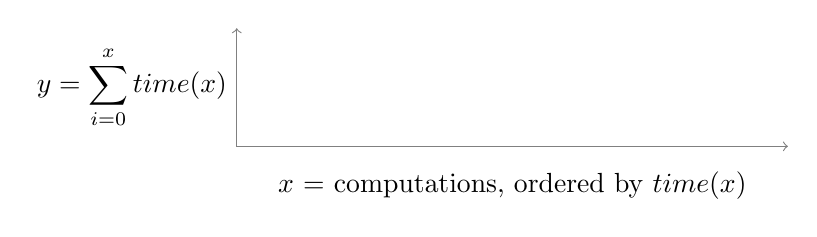
\begin{tikzpicture}
	%\draw[step=1,gray,very thin] (0,0) grid (10,3);
	\draw[<->,gray,thin] (0,1.5) -- (0,0.75) node [black,anchor=east] {$\displaystyle y = \sum_{i=0}^{x} time(x)$}-- (0,0) -- (7,0);
	\node at (3.5,-0.5) {$x$ = computations, ordered by $time(x)$};
	\draw[blue!50!gray,thick] plot file {chap-algorithms/data-cumulative-baseline-timing};
\end{tikzpicture}

	\end{center}}
	\figpostamble
	\caption{Cumulative time required for collocation computations.}
	\label{fig:cumulative-baseline-timing}
\end{figure}

\figpreamble
\begin{figure}
	\figfontsize{
	\begin{center}
		\begin{tikzpicture}
	%\draw[step=1,gray,very thin] (0,0) grid (10,3);
	\draw[<->,gray,thin] (0,1.5) -- (0,0.75) node [black,anchor=east] {$y=\log time$}-- (0,0) -- (7,0);
	\node at (3.5,-0.5) {$x = \log (|Q_{w_1 X ... X w_k}| + |Q_{w_{k+1}}|)$};
	\draw plot[only marks,mark=*,mark options={color=blue!50!gray},mark size=0.5pt] file {chap-algorithms/data-scatterplot-baseline-timing};
\end{tikzpicture}

	\end{center}}
	\figpostamble
	\caption{Size of input sets ($|M_1^k| + |M_{k+1}|$) compared with time required to compute collocation from the two sets using the baseline algorithm (double logscale).}
	\label{fig:scatterplot-baseline}
\end{figure}

\noindent Our solution addresses both of these problems.  We
introduce an algorithm for efficient enumeration that performs 
lossless pruning of unnecessary queries
(\textsection\ref{sec:efficient-enumeration}).  We also introduce
several strategies to reduce the cost of individual queries
(\textsection\ref{sec:efficient-lookup})

\subsection{Efficient Enumeration}
\label{sec:efficient-enumeration}

Although we found 2895 query patterns per sentence,
the average sentence length is just over 29 words.
Obviously, the query patterns are highly overlapping.
We can exploit this to reduce computational expense.

\subsubsection{The Zhang-Vogel Algorithm}\label{sec:zhang-vogel}

\citet{Zhang:2005:eamt} show an efficient algorithm
for contiguous phrase searches in a suffix array.  It is based
on the observation that the prefix $u$ of any possible
source phrase $ua$ is itself a possible source
phrase.  They exploit this fact to reduce the amount of work required
to search for $ua$.  The set of suffixes with prefix $ua$ is
a subset of the set of suffixes with prefix $u$.
Therefore, if we search for occurrences of
$u$ before searching for occurrences of $ua$, we can
restrict the binary search for $ua$ to the suffix array range
containing suffixes prefixed by $u$.
If there are no matches for $u$, we
don't need to search for $ua$ at all.  
This optimization improves efficiency for
phrase search, although the improvement is
modest since search for contiguous phrases
is already very fast
(\textsection\ref{sec:overview-results}).\footnote{
In fact, the results reported 
in the previous chapter incorporate both
this optimization and one we introduce in 
\textsection\ref{sec:zv-improvements}.}
However, the opportunity for improvement in discontiguous search
is much greater.  

Extension to hierarchical
phrases is straightforward.  A hierarchical
phrase $\alpha{}a$ can only occur in $T$ if its
prefix $\alpha$ occurs in $T$.  The actual pattern matching
algorithm for hierarchical phrases is not as simple
as binary search in a suffix array, so this doesn't
enable an obvious search improvement as it does for
contiguous phrases.  However, it does allow us to rule out the 
existence of $\alpha{}a$ if the search for $\alpha$
fails.  This prunes out many searches
that are guaranteed to be fruitless.

\subsubsection{Prefix Trees and Suffix Links}\label{sec:zv-improvements}

The Zhang-Vogel optimization is closely related to
prefix trees.  Recall that the prefix tree implementation of a phrase
table encodes all legal source phrases in an unminimized 
finite state automaton (\textsection\ref{sec:phrase-tables}).  
We store target phrases and scores
at the node associated with a source phrase.
Representing hierarchical rules in the prefix tree
requires no special modification.  Since our nonterminal
and terminal alphabets are mutually exclusive, we simply
treat the nonterminal $X$ as any other edge 
label.\footnote{Conveniently, the decoder used in our
experiments \citep{Chiang:2007:cl} already encodes its
grammars in a prefix tree.  The implementation is 
similar to one described by \citet{Klein:2001:acl}.  We
simply augment this representation with information
needed by our algorithms.}

We implement the Zhang-Vogel algorithm using
a prefix tree, which we construct for each source
sentence.  In fact, we can think of the pattern
matching operation itself as an augmentation of edge 
traversal in a prefix tree.  Suppose that we are at a
node representing source phrase $\alpha$, and we want to 
find translation rules for source phrase $\alpha{}a$.  
If the node representing $\alpha$ does not have
an outgoing $a$-edge, we first query the source text for
phrase $\alpha{}a$.  If the query succeeds, we add an
$a$-edge to a new node containing the newly extracted
phrase pairs and scores.  If the search fails, we still
add the $a$-edge, but we mark the new node as {\em inactive},
indicating that the text contains no phrases with this prefix.
In this way, the algorithm builds a prefix
tree representing every query pattern licensed by our grammar
for the input sentence, except patterns whose prefixes were
not present in the training data (Figure~\ref{fig:prefix-tree}).
Now suppose that a source phrase occurs multiple times
in the sentence (this frequently happens with determiners for example).
The first occurrence is treated as described above, but
for all subsequent occurrences we simply traverse the existing edge.
We check the flag on the node to see if it is active or inactive,
telling us whether the previous
search was successful.  Recall that the prefix tree is 
sentence-specific.  We discard it and build a new tree for 
each sentence, enabling our decoder to run indefinitely 
without exhausting main memory.

\figpreamble
\begin{figure}
	\figfontsize{
	\begin{center}
		\begin{tikzpicture}[level distance=2.5cm]
	\tikzstyle{edge from parent} = [->,draw]
	\tikzstyle{level 1} = [sibling distance=5cm]
	\tikzstyle{level 2} = [sibling distance=3cm]
	\tikzstyle{level 3} = [sibling distance=1cm]
	\tikzstyle{level 4} = [sibling distance=1cm]
	\clip (-0.2,-4.25) rectangle (15,6);
	\node (a legend)[active node] at (10,-3) {}; \node (a legend text)[anchor=west] at (a legend.east) {active node};
	\node (i legend)[inactive node] at (10,-3.5){}; \node (i legend text) [anchor=west] at (i legend.east) {inactive node};
	\path (a legend.north west) -- +(-3pt,3pt) coordinate (legend box top);
	\draw [gray,thin](legend box top) rectangle (i legend text.south east);
	\node [root node]{}[grow'=right]
		child {node [active node]{} edge from parent node [below=2.5cm,left=0.7cm]{it}} 
		child {node [inactive node]{} edge from parent node [right]{persuades}} 
		child {node [active node]{}{
			child {node [active node]{}{
				child [sibling distance=2cm]{node [active node]{}{
					child {node [inactive node]{} edge from parent node [above=1mm]{disheartens}} 
					child {node [active node]{}{
						child {node [active node]{} edge from parent node [above]{him}} 
						} edge from parent node [below]{X}} 
					} edge from parent node [above=1mm]{it}}
				child {node [active node]{}{
					child {node [active node]{} edge from parent node [above]{him}} 
					child {node [inactive node]{} edge from parent node [below]{disheartens}} 
					} edge from parent node [below]{X}}
				} edge from parent node [above=1mm]{and}}
			child {node [active node]{}{
				child {node [active node]{}{
					child {node [inactive node]{} edge from parent node [above]{disheartens}} 
					child {node [active node]{}{
						child {node [active node]{} edge from parent node [above]{him}} 
						} edge from parent node [below]{X}} 
					} edge from parent node [above]{it}}
				child {node [inactive node]{} edge from parent node [above=4mm,right=1mm]{disheartens}} 
				child {node [active node]{} edge from parent node [below]{him}} 
				} edge from parent node [below]{X}}
			} edge from parent node [above=3mm]{him}} 
		child {node [active node]{}{
			child  [sibling distance=2cm] {node [active node]{}{
				child {node [inactive node]{} edge from parent node [above=1mm]{disheartens}} 
				child {node [active node]{}{
					child {node [active node]{} edge from parent node [above]{him}} 
					} edge from parent node [below]{X}} 
				} edge from parent node [above]{it}}
			child  [sibling distance=2cm]  {node [active node]{}{
				child {node [active node]{} edge from parent node [above]{him}} 
				child {node [inactive node]{} edge from parent node [below]{disheartens}} 
				} edge from parent node [below]{X}}
			} edge from parent node [below=3mm]{and}} 
		child {node [inactive node]{} edge from parent node [right]{disheartens}} 
		child {node [active node]{} edge from parent node [above=2.5cm,left=0.7cm]{X}}; 
\end{tikzpicture}
	\end{center}}
	\figpostamble
	\caption{Portion of the prefix tree for tree for our example input (Figure~\ref{fig:hiero-query}).}
	\label{fig:prefix-tree}
\end{figure}

We can improve on the Zhang-Vogel algorithm.
The existence of phrase $a\alpha{}b$ in a text
guarantees more than the existence of its prefix
$a\alpha$.  It also guarantees the existence of
its suffix $\alpha{}b$.  If $\alpha{}b$ doesn't exist,
we don't need search for $a\alpha{}b$ at all.  
Furthermore, note that unless $\alpha=X$, $a\alpha$ and
$\alpha{}b$ must share at least one word.  This means
we can reduce the search to cases where $a\alpha$ and 
$\alpha{}b$ overlap, and their starting indices will differ
by exactly one.  To see why this
is useful, consider a phrase $abXcd$.   In our 
baseline algorithm, we would search for $ab$ and 
$cd$, and then perform a computation to see whether these
subphrases were collocated within an elastic window.
However, if we instead use the locations of $abXc$ and $bXcd$ as the basis
of the computation, we gain two advantages.  First, the
number of elements in each set is likely to be smaller than
in the former case.  This is not guaranteed to be true, but
it will be true in the vast majority of cases.\footnote{
To see why this isn't always the case, consider an example.
Suppose that our subpatterns are $ab$ and $cd$, and the 
text contains the substring $ababdcdcd$.  Although each
subpattern occurs only twice, the combined pattern $abXcd$
occurs four times.}
Second, the computation becomes
simpler because there is no need to check whether
the patterns cooccur within a variable-length window.
It is sufficient to see whether they match exactly,
except for the first index, which should differ by 
exactly one.  For this to work, we need
access to the set of locations for both the
prefix and the suffix.  Note that any
pattern $\alpha$ can be the prefix or suffix of numerous source
phrases.  To facilitate reuse of the
occurrence set $M_\alpha$, we cache it at the
corresponding prefix tree node.  The full algorithm
for computing occurrences $a\alpha{}b$ given all
occurrences of $a\alpha$ and $\alpha{}b$ will be described
in \textsection\ref{sec:collocation-algorithm}.

To access suffixes in constant time, we augment
the prefix tree with {\em suffix links}.  A suffix link 
is a pointer from a node representing $a\alpha{}b$ to a node 
representing its suffix $\alpha{}b$ (Figure~\ref{fig:prefix-tree-suffix-links}).
Via this connection, we can immediately check to see if 
the node has been marked inactive.  If it is, we know that a query
for the $\alpha{}b$ (or recursively, one of its suffixes) previously
failed, and we don't need to query for $a\alpha{}b$ at all, since
we know that it will not be found.\footnote{Note that the suffix 
of a one-symbol phrase is the empty string $\epsilon$, represented 
by the root node of the prefix tree.  The reader may notice 
that $a\alpha$ is undefined when the prefix pattern is 
$\epsilon$.  We define an auxiliary state $\perp$, 
following \citet{Ukkonen:1995:algorithmica}.  The suffix link from root
points to $\perp$, while $\perp$ is connected to the root node 
by all symbols in the alphabet.  Therefore, when $\alpha = \epsilon$,
$a\alpha = \perp$.  Following the $a$-edge from $\perp$ 
returns us to the root.  This simplifies much of the following
algorithmic discussion without requiring the enumeration of several
corner cases.}

\figpreamble
\begin{figure}
	\figfontsize{
	\begin{center}
		\begin{tikzpicture}[level distance=2.5cm]
	\tikzstyle{suffix link} = [->,densely dotted]
	\tikzstyle{level 1} = [sibling distance=2.5cm]
	\tikzstyle{level 2} = [sibling distance=2cm]
	\tikzstyle{level 3} = [sibling distance=1cm]

	%\clip (-1,-3.5) rectangle (14,6);
	\tikzstyle{edge from parent} = [->,draw]
	\node (root)[root node]{}[grow'=right]
		child [sibling distance=2cm]{node (him)[active node]{} edge from parent node [left]{him}}
		child {node (it)[active node]{}{
			child [sibling distance=1cm]{node (it disheartens)[inactive node]{} edge from parent node [above=1mm]{disheartens}} 
			child [sibling distance=1cm]{node (it X)[active node]{}{
				child {node (it X him)[active node]{} edge from parent node [above]{him}} 
				} edge from parent node [below]{X}} 
			} edge from parent node [below]{it}}
		child {node (and) [active node]{}{
			child {node (and it)[active node]{}{
				child {node (and it disheartens)[inactive node]{} edge from parent node [above=1mm]{disheartens}} 
				child {node (and it X)[active node]{}{
					child {node (and it X him)[active node]{} edge from parent node [above]{him}} 
					} edge from parent node [below]{X}} 
				} edge from parent node [above]{it}}
			child  {node (and X)[active node]{}{
				child {node (and X him) [active node]{} edge from parent node [above]{him}} 
				child {node (and X disheartens)[inactive node]{} edge from parent node [below]{disheartens}} 
				} edge from parent node [below]{X}}
			} edge from parent node [above]{and}}
		child  {node (X)[active node]{}{
			child [sibling distance=1cm]{node (X him)[active node]{} edge from parent node [above]{him}} 
			child [sibling distance=1cm]{node (X disheartens)[inactive node]{} edge from parent node [below]{disheartens}} 
			} edge from parent node [below]{X}}
		child [sibling distance=2cm]{node (disheartens)[inactive node]{} edge from parent node [left=5mm,below=3mm]{disheartens}} 
			
		;
	\draw[suffix link] (and X) ..controls +(-1.5,-0.5) .. (X.north);
	\draw[suffix link] (X disheartens) ..controls +(-0.75,-0.75) .. (disheartens);
	\draw[suffix link] (and X disheartens) ..controls +(-0.5,-1) .. (X disheartens);
	\draw[suffix link] (and X him) ..controls +(2,-1) and +(2,-1).. (X him);
	\draw[suffix link] (disheartens) ..controls +(-2.5,0) and +(-1.5,-2) .. (root);
	\draw[suffix link] (X) ..controls +(0,1) .. (root);
	\draw[suffix link] (and) ..controls +(0,-1) .. (root);
	\draw[suffix link] (it) ..controls +(0,-1.5) and +(1.5,0.5).. (root);
	\draw[suffix link] (and it) ..controls +(-2,0) .. (it);
	\draw[suffix link] (and it X) ..controls +(2,3) and +(1,1).. (it X);
	\draw[suffix link] (and it X him) ..controls +(-0.5,1.5).. (it X him);
	\draw[suffix link] (and it disheartens) ..controls +(2,2) and +(2,1).. (it disheartens);
	\draw[suffix link] (it disheartens) .. controls +(9,1) and +(9,0) .. (disheartens);
	
%	\node (him) [rectangle, draw] at (1,5) {};
%	\draw[->] (root) -- (him) node [pos=0.5,left] {him};
	\draw[suffix link] (him) ..controls +(-1.5,0) and +(-1,3) .. (root);
	\draw[suffix link] (X him) .. controls +(10,-1) and +(10,3) .. (him);
	
%	\node (him plus) at (3,7) {};
%	\node (him plus plus) at (3,9) {};
%	\draw[->] (him) -- (him plus);
%	\draw[->] (him) -- (him plus plus);
%
%	\node (it plus) at (4,7) {};
%	\node (it plus plus) at (4,9) {};
%	\draw[->] (it) -- (it plus);
%	\draw[->] (it) -- (it plus plus);
%

\end{tikzpicture}
	\end{center}}
	\figpostamble
	\caption[A fragment of the prefix tree augmented with suffix links.]{A fragment of the prefix tree (Figure~\ref{fig:prefix-tree}) augmented with suffix links (dotted).}
	\label{fig:prefix-tree-suffix-links}
\end{figure}

As we described above, the prefix tree acts as a cache 
for phrases that occur multiple
times in a source sentence.  In these cases, we simply
traverse the already-constructed edge, without needing to
query the text for the phrase or extract its translations.  Depending on our usage
scenario and available memory, we could extend the caching 
behavior even further by retaining part or all of the tree 
between sentences instead of building a new tree for 
each sentence.  For instance, a least recently used (LRU)
strategy for cache pruning may improve translation speed for whole
documents without exhausting memory.  Though impractical for online settings,
in batch translation we could simply keep the
entire tree for the duration of the decoding process.  This
allows us to reuse queries that were already performed for
previous sentences, potentially leading to further speedups.

\subsubsection{Special Cases for Phrases with Gaps}\label{sec:special-cases}

The model permits gaps at the beginning or end of a hierarchical phrase.
For instance, it permits source phrases $Xu$ or $uX$ or even $XuX$.
However, even if our model disallowed such source phrases, they would still
be prefixes or suffixes of valid sources sources, and therefore must
appear in the prefix tree.  Each of these phrases corresponds to a 
unique path in the prefix tree, although 
for pattern matching purposes they are all identical to phrase $u$.
An analogous situation occurs with the patterns $XuXv$, $uXvX$, 
and $uXv$.  There are two cases that we are concerned with.

Consider a pattern $\alpha = X\beta$.  The path to its prefix 
tree node contains the $X$-edge originating at the root
node.  All paths containing this edge form a special subtree.
Note that $\alpha$ occurs in the text at the same locations as
$\beta$, although from the perspective of the translation model
it is a different phrase.  Therefore, we don't actually
need to query the training text to find $\alpha$.  If the node 
representing $\beta$ is active, we create an active node 
for $\alpha$ and set $M_\alpha = M_\beta$.  If the node 
representing $\beta$ is inactive, we create an inactive node for $\alpha$.

Now consider pattern $\alpha = \beta{}X$.  For pattern matching purposes,
this pattern is identical to its prefix $\beta$.
Therefore, if we successfully find $\beta$, we automatically
add an outgoing $X$-edge from its corresponding node,
provided that $\beta{}X$ is licensed  
by the length restrictions.  Again we set $M_\alpha = M_\beta$.

Note that both special cases occur for a pattern in the form $\alpha = X\beta{}X$.

\subsubsection{Putting It All Together: Prefix Tree Generation Algorithm}\label{sec:prefix-trees}

Given an input sentence, our algorithm (Listing~\ref{alg:prefix-tree})
generates the corresponding prefix tree for its query patterns breadth-first.
We maintain a queue of items, each consisting of a
query pattern, its span in the input, and a pointer to the node 
corresponding to its prefix.  The queue is initialized
with all patterns containing a single terminal symbol.  When we
pop a pattern from the queue, there are two cases.  If the
corresponding edge exists in the prefix tree,
we traverse it.  Otherwise, we query the source text for 
the pattern.  Irrespective of the query's success, 
we create a node for the pattern in the tree, and
mark it active or inactive as appropriate.  For found patterns, we 
cache either the endpoints of the suffix array range containing
the phrase (if it is contiguous), or the full list of locations at which
the phrase is found (if it is discontiguous).\footnote{As a practical
matter, we can also store the scored translation rules after we extract
them (\textsection\ref{sec:hierarchical-extraction}).}
We add to the queue any query patterns 
containing one more terminal for which the pattern is a prefix.  
This guarantees that all patterns containing $m$ terminals
are processed before any patterns containing $m+1$ terminals,
which is sufficient to guarantee that any pattern is processed
after both its suffix and prefix.

To query the text for pattern $a\alpha{}b$, we 
call function \queryfunc\ (\textsection\ref{sec:collocation-algorithm}), providing 
the sets of prefix and suffix locations
$M_{a\alpha}$ and $M_{\alpha{}b}$ as parameters.  $M_{a\alpha}$ is
cached at the node corresponding to the prefix $a\alpha{}$, 
which is an element of the item popped from the queue.
To find the node corresponding to the suffix $\alpha{}b$, 
we first follow the suffix link from the node representing 
the prefix, $a\alpha$.  This leads us to a node representing
$\alpha$.  From this node we follow the $b$-edge, which
leads to the node representing $\alpha{}b$.  This 
gives us constant-time access to both prefix and suffix information.
If the suffix node is inactive, we can
mark the new node inactive without a query.
Some common cases are illustrated
in Figure~\ref{fig:prefix-tree}.

\algorithm{Prefix Tree Lookup}{
	\label{alg:prefix-tree}
	
\newcommand\varsuffix{\mathit{suffix}}
\newcommand\varprefix{\mathit{prefix}}
\newcommand\funcchildren{\mathrm{children}}

\newcommand\sufflink{\mathit{suffix\_link}}

\noindent {\bf Function} {\sc Generate\_Prefix\_Tree}

\noindent {\bf Input:} source sentence $f_1^I$, prefix tree root node $p_\epsilon$
\begin{algorithmic}[1]

	\State $\funcchildren(p_\epsilon) \leftarrow \funcchildren(p_\epsilon) \cup p_X$
	\For {$i$ from $1$ to $I$}
		\State Add $\langle f_i,i,i+1,p_\epsilon \rangle$ to queue \Comment $\langle$pattern, span start, span end, prefix node$\rangle$
	\EndFor
	\For {$i$ from 1 to $I$}
		\State Add $\langle Xf_i, i-1, i+1, p_X \rangle$ to queue
	\EndFor
	\While {queue is not empty}
		\State Pop $\langle \alpha, i, j, p_{a\beta} \rangle$ from queue
		\If {$p_{a\beta{}f_j} \in \funcchildren(p_{a\beta})$}
			\If{$p_{a\beta{}f_j}$ is inactive}
				\State Continue to next item in queue
			\Else
				\State \Call{Extend\_Queue}{$a\beta{}f_j, i, j, f_1^I$}
			\EndIf
		\Else
			\State $\funcchildren(p_{a\beta}) \leftarrow \funcchildren(p_{a\beta}) \cup p_{a\beta{}f_j}$
			\State $p_\beta{} \leftarrow \sufflink(p_{a\beta})$
			\If {$p_{\beta{}f_j}$ is inactive}
				\State Mark $p_{a\beta{}f_j}$ inactive
			\Else
				\State $Q_{a\beta{}f_j} \leftarrow$ \Call{Query}{$a\beta{}f_j, Q_{a\beta}, Q_{\beta{}f_j}$}
				\If {$Q_{a\beta{}f_j} = \emptyset$}
					\State Mark $p_{a\beta{}f_j}$ inactive
				\Else
					\State Mark $p_{a\beta{}f_j}$ active
					\State \Call{Extend\_Queue}{$a\beta{}f_j, i, j, f_1^I$}
				\EndIf
			\EndIf
		\EndIf
	\EndWhile

\end{algorithmic}

~

\noindent {\bf Function} {\sc Extend\_Queue}

\noindent {\bf Input:} $\alpha, i, j, f_1^I, p_\alpha$
\begin{algorithmic}[1]
	\If {$|\alpha| < \maxphraselen$ and $j-i+1 \leq \maxphrasespan$}
		\State Add $\langle \alpha{}f_j, i, j+1, p_\alpha \rangle$ to queue
		\If {$arity(\alpha) < \maxnts$}
			\State $\funcchildren(p_{\alpha}) \leftarrow \funcchildren(p_{\alpha}) \cup p_{\alpha{}X}$
			\State Mark $p_{\alpha{}X}$ active
			\State $Q_{\alpha{}X} \leftarrow Q_\alpha$ 
			\For{$k$ from $j+1$ to $min(I,i+\maxphraselen)$}
				\State Add $\langle \alpha{}f_jXf_k, i, k, \alpha{}X \rangle$ to queue
			\EndFor
		\EndIf
	\EndIf
\end{algorithmic}

%	for k, i, node, prefix, is_shadow_path in frontier:
%
%		word_id = fwords[i]
%		phrase = prefix + (word_id,)
%		str_phrase = map(sym.tostring, phrase)
%		hiero_phrase = rule.Phrase(phrase)
%		arity = hiero_phrase.arity()
%
%		#log.writeln("pos %2d, node %5d, '%s'" % (i, node.id, hiero_phrase), 3)
%		if self.search_file is not None:
%			self.search_file.write("%s\n" % hiero_phrase)
%
%		lookup_required = False
%		if word_id in node.children:
%			if node.children[word_id] is None:
%				#log.writeln("Path dead-ends at this node", 4)
%				continue
%			else:
%				#log.writeln("Path continues at this node", 4)
%				node = node.children[word_id]
%		else:
%			if node.suffix_link is None:
%				#log.writeln("Current node is root; lookup required", 4)
%				lookup_required = True
%			else:
%				if word_id in node.suffix_link.children:
%					if node.suffix_link.children[word_id] is None:
%						#log.writeln("Suffix link reports path is dead end", 4)
%						node.children[word_id] = None
%						continue
%					else:
%						#log.writeln("Suffix link indicates lookup is reqired", 4)
%						lookup_required = True
%				else:
%					#log.writeln("ERROR: We never get here")
%					raise Exception("Keyword trie error")
%

}

\figpreamble
\begin{figure}
	\figfontsize{
	\begin{center}
		\begin{tikzpicture}[level distance=2cm,node distance=1.5cm]
	\tikzstyle{level 1} = [sibling distance=1cm]

	\tikzstyle{edge from parent} = [->,draw]
	\node (root)[root node]{}[grow'=right]
		child  {node (X) [active node]{}{
			child {node (X disheartens) [inactive node]{} edge from parent node [above]{disheartens}} 
			} edge from parent node [above]{X}}
		child {node (it)[active node]{}{
			child {node (it X)[active node]{}{
				} edge from parent node [below]{X}} 
			} edge from parent node [below]{it}}
		;

	\draw[suffix link] (X) ..controls +(-0.75,0.75) and +(0,0.75) .. (root);
	\draw[suffix link] (it) ..controls +(-0.5,0.5) .. (root);
	\draw[suffix link] (it X.north) -- (X.south);

	\node [anchor=south,above of=X,node distance=1cm] {Queue: it X disheartens};
	\node [anchor=north,below of=it,text centered,text width=7cm] {Case 1. Queue item not in tree, suffix node is inactive.};
	
	\node (root) at (6,0)[root node]{}[grow'=right]
		child  {node (X) [active node]{}{
			child {node (X disheartens) [inactive node]{} edge from parent node [above]{disheartens}} 
			} edge from parent node [above]{X}}
		child {node (it)[active node]{}{
			child {node (it X)[active node]{}{
				child {node (it X disheartens) [inactive node]{} edge from parent node [below]{disheartens}}
				} edge from parent node (X label)[below]{X}} 
			} edge from parent node [below]{it}}
		;

	\draw[suffix link] (X) ..controls +(-0.75,0.75) and +(0,0.75) .. (root);
	\draw[suffix link] (it) ..controls +(-0.5,0.5) .. (root);
	\draw[suffix link] (it X.north) -- (X.south);
	\draw[suffix link] (it X disheartens.north) -- (X disheartens.south);

	\node (center point) at (X label.north){};
	\node [anchor=north,below of=center point,text centered,text width=7cm] {Result. Node added as inactive without search, nothing added to queue.};

	\draw[thin,gray] (-1,-2.75) -- +(14,0);

	\begin{scope}[yshift=-4.6cm]

		\node (root)[root node]{}[grow'=right]
			child {node (X)[active node]{}{
				child {node (X it)[active node]{}{} edge from parent node [above]{it}} 
				} edge from parent node [above]{X}}
			child  {node (him) [active node]{}{
				child {node (him X) [active node]{} edge from parent node [below]{X}} 
				} edge from parent node [below]{him}}
			;

		\draw[suffix link] (X) ..controls +(-0.75,0.75) and +(0,0.75) .. (root);
		\draw[suffix link] (him) ..controls +(-0.5,0.5) .. (root);
		\draw[suffix link] (him X.north) -- (X.south);

		\node [anchor=south,above of=X,node distance=1cm] {Queue: him X it};
		\node [anchor=north,text centered,text width=4cm] at (1.5,-2.5) {Case 2. Queue item not in tree, suffix node is active, and pattern occurs in text.};

		\matrix (him locations) [nodes={minimum width=6.5mm,minimum height=6mm,rectangle,draw},anchor=north] at (3.75,-2) {
			\node (2) {2}; \\
			\node (15) {15}; \\
			\node (10) {10}; \\
			\node (6) {6}; \\
		};
		\path[fill=lightgray] (him X.center) -- (2.north east) -- (2.north west) -- cycle;

		\matrix (it locations) [nodes={minimum width=6.5mm,minimum height=6mm,rectangle,draw},anchor=north] at (5.25,-2) {
			\node (0) {0}; \\
			\node (4) {4}; \\
			\node (8) {8}; \\
			\node (13) {13}; \\
		};

		\path[fill=lightgray] (X it.center) -- (13.south west) -- (0.north west) -- (0.north east) -- cycle;
		\node [anchor=south east] at (him locations.north) {$M_\mathrm{him~X}$};
		\node [anchor=south west] at (it locations.north) {$M_\mathrm{X~it}$};

		\draw[<->] (2.east) -- (4.west);
		\draw[<->] (2.east) -- (8.west);
		\draw[<->] (2.east) -- (13.west);
		\draw[<->] (10.east) -- (13.west);
		\draw[<->] (6.east) -- (8.west);
		\draw[<->] (6.east) -- (13.west);

		\draw[snake=brace,raise snake=1mm,segment amplitude=2mm] (0.north east) -- (13.south east);
		\path (4.south east) -- +(3mm,0) coordinate (arrow start);

		\matrix (result locations) [nodes={minimum width=12mm,minimum height=6mm,rectangle,draw},anchor=west,right of=it locations,node distance=2cm] {
			\node (result top){$2,4$}; \\
			\node {$2,8$}; \\
			\node (result side){$2,13$}; \\
			\node {$10,13$}; \\
			\node {$6,8$}; \\
			\node (result bottom){$6,13$}; \\
		};
		\draw[->] (arrow start) -- (result side.south west);

		\node (root) at (6,0)[root node]{}[grow'=right]
			child {node (X)[active node]{}{
				child {node (X it)[active node]{}{} edge from parent node (it label) [above]{it}} 
				} edge from parent node [above]{X}}
			child  {node (him) [active node]{}{
				child {node (him X) [active node]{}{
					child {node (him X it) [active node] {} edge from parent node [below]{it}}
					} edge from parent node [below]{X}} 
				} edge from parent node [below]{him}}
			;

		\node (agenda loc) at (it label.south) {};
		\node [anchor=south,above of=agenda loc,node distance=1cm] {Queue: him X it disheartens, him X it X him};

		\draw[suffix link] (X) ..controls +(-0.75,0.75) and +(0,0.75) .. (root);
		\draw[suffix link] (him) ..controls +(-0.5,0.5) .. (root);
		\draw[suffix link] (him X.north) -- (X.south);
		\draw[suffix link] (him X it.north) -- (X it.south);

		\draw[snake=brace,raise snake=1mm,segment amplitude=2mm,segment aspect=0.166] (result top.north east) -- (result bottom.south east);
		\path (result top.south east) -- +(3mm,0) coordinate (arrow start);
		\draw[->] (arrow start) ..controls (arrow start -| him X it.south) .. (him X it.south);

		\node [anchor=north,text centered,text width=5cm] at (10.5,-2.5) {Result. Compute $M_{him~X~it}$ from $M_{him~X}$ and $M_{X~it}$, store in new active node, and add subsequent patterns to queue.};

		\draw[thin,gray] (-1,-5.5) -- +(14,0);

	\end{scope}

	\begin{scope}[yshift=-12cm]

		\node (root)[root node]{}[grow'=right,level distance=1.33cm]
			child {node (X)[active node]{}{
				child {node (X him) [active node]{}{
					child {node (X him and) [active node]{}{
						} edge from parent node [above]{and}}
					} edge from parent node [above]{him}}
				} edge from parent node [above]{X}}
			child  {node (and) [active node]{}{
				child {node (and X) [active node]{}{
					child {node (and X him)[active node]{}{
						} edge from parent node [below]{him}}
					} edge from parent node [below]{X}} 
				} edge from parent node [below]{and}}
			;
			
		\draw[suffix link] (X) ..controls +(-0.75,0.75) and +(0,0.75) .. (root);
		\draw[suffix link] (and) ..controls +(-0.5,0.5) .. (root);
		\draw[suffix link] (and X.north) -- (X.south);
		\draw[suffix link] (and X him.north) -- (X him.south);
		
		\node [anchor=south,above of=X him,node distance=1cm] {Queue: and X him and};
		\node [anchor=north,text centered,text width=4cm] at (1.5,-2) {Case 3. Queue item not in tree, suffix node is active, but pattern does not occur in text.};

		\matrix (X him and locations) [nodes={minimum width=6.5mm,minimum height=6mm,rectangle,draw},anchor=north] at (5.75,-2) {
			\node (2) {2}; \\
		};

		\matrix (and X him locations) [nodes={minimum width=12mm,minimum height=6mm,rectangle,draw},anchor=north] at (4.25,-2) {
			\node (loc 1){$3,6$}; \\
			\node (loc 2){$3,10$}; \\
			\node (loc 3){$12,15$}; \\
		};

		\path[fill=lightgray] (X him and.center) -- (2.south west) -- (2.north west) -- (2.north east) -- cycle;
		\path[fill=lightgray] (and X him.center) -- (loc 1.north east) -- (loc 1.north west) --cycle;

		\node [anchor=south east] at (and X him locations.north) {$M_\mathrm{and~X~him}$};
		\node [anchor=south west] at (X him and locations.north) {$M_\mathrm{X~him~and}$};

		\draw[snake=brace,raise snake=1.35cm,segment amplitude=2mm] (loc 1.north east) -- (loc 3.south east);
		\node [anchor=west,right=1.5cm] at (loc 2.east) {$\emptyset$};


		\node (root) [root node] at (6,0){}[grow'=right,level distance=1.33cm]
			child {node (X)[active node]{}{
				child {node (X him) [active node]{}{
					child {node (X him and) [active node]{}{
						} edge from parent node [above]{and}}
					} edge from parent node [above]{him}}
				} edge from parent node [above]{X}}
			child  {node (and) [active node]{}{
				child {node (and X) [active node]{}{
					child {node (and X him)[active node]{}{
						child {node (and X him and)[inactive node]{}{
							} edge from parent node [below]{and}}
						} edge from parent node [below]{him}}
					} edge from parent node [below]{X}} 
				} edge from parent node [below]{and}}
			;
			
		\draw[suffix link] (X) ..controls +(-0.75,0.75) and +(0,0.75) .. (root);
		\draw[suffix link] (and) ..controls +(-0.5,0.5) .. (root);
		\draw[suffix link] (and X.north) -- (X.south);
		\draw[suffix link] (and X him.north) -- (X him.south);
		\draw[suffix link] (and X him and.north) -- (X him and.south);

		\node [anchor=north,text centered,text width=5.5cm] at (10,-2) {Result. Computation finds that pattern is not present. Add inactive node.};

	\end{scope}


\end{tikzpicture}
	\end{center}}
	\figpostamble
	\caption{Illustration of several recursive cases in the prefix tree construction algorithm.}
	\label{fig:prefix-tree-recursive-cases}
\end{figure}


\theoremstyle{definition}
\newtheorem{definition}{Definition}

\subsubsection{The Basic \queryfunc\ Algorithm}
\label{sec:collocation-algorithm}

We need to define function \queryfunc\ called
by the prefix tree algorithm (Listing~\ref{alg:prefix-tree}).
Its input consists of set $M_{a\alpha}$ representing all
{\em matchings} of prefix $a\alpha$ and set $M_{\alpha{}b}$ representing all
matchings of suffix $\alpha{}b$.  From this it must compute 
all matchings $M_{a\alpha{}b}$ of query pattern $a\alpha{}b$.

Recall from \textsection\ref{sec:baseline} that
a matching in the text for pattern 
$\alpha = w_1 X ... X w_{K_\alpha}$ is a $K_\alpha$-tuple 
$m_\alpha = (m_{\alpha,1}, ..., m_{\alpha,K_\alpha})$. 
The $k$th element $m_{\alpha,k}$ of $m_\alpha$ is the starting index
of a substring in $T$ matching subpattern $w_k$.  If two patterns
differ only by preceding or following nonterminal symbol $X$, then
their matchings in $T$ are identical.  More formally, 
if $\alpha = \beta{}X$ or $\alpha = X\beta$ then 
$M_\alpha = M_\beta$.  If $\alpha = X$
then $M_\alpha = ()$, the empty tuple.

For the discussion that follows, we will find it useful to 
define several formal properties of matchings.  First, we define an ordering.
For matchings $m_\alpha$ and $m_\alpha'$ of pattern $\alpha$,
$m_\alpha < m_\alpha'$ if and only if $\exists_{k \in \{1,...,K_\alpha\}} (m_{\alpha,k} < m'_{\alpha,k}$ and $\forall_{\ell \in \{1,...,k-1\}}  m_{\alpha,\ell} = m'_{\alpha,\ell})$.
Thus, a set of $K_\alpha$-tuples is ordered on the first index, 
then the second, and so on.

The {\em suffix matching} $s(m_{a\alpha})$ of 
matching $m_{a\alpha}$ is 
the embedded matching of suffix $\alpha$.
If $\alpha = X\beta$ and $m_{\alpha} = s(m_{a\alpha{}})$
then $K_{\alpha} = K_{a\alpha}-1$ and
$m_\alpha = (m_{a\alpha,2},...,m_{a\alpha,K_{a\alpha}})$.
If $\alpha = \beta{}c$ and $m_{\alpha} = s(m_{a\alpha{}})$
then $K_{\alpha,1} = K_{a\alpha,1}+1$, $m_{\alpha,1} = m_{a\alpha,1}+1$ and 
$\forall_{k \in \{2,...,K_{\alpha}\}} m_{\alpha,k} = m_{a\alpha,k}$.

The relationship between a matching and its suffix matching are shown in Figure~\ref{fig:matching-relationships}.

Analogously, the {\em prefix matching} $p(m_{\alpha{}b})$ of 
matching $m_{\alpha{}b}$ of pattern $\alpha{}b$ is 
the embedded matching of its prefix $\alpha$.
If $\alpha = \beta{}X$ and $m_{\alpha} = p(m_{\alpha{}b})$
then $K_{\alpha} = K_{\alpha{}b}-1$ and 
$m_\alpha = (m_{\alpha{}b,1},...,m_{\alpha{}b,K_{\alpha}})$.
If $\alpha = \beta{}c$ and $m_{\alpha} = p(m_{\alpha{}b})$
then $K_{\alpha} = K_{\alpha{}b}$ and $m_{\alpha} = m_{\alpha{}b}$.

\figpreamble
\begin{figure}
	\figfontsize{
	\begin{center}
		\begin{tikzpicture}
	\matrix (text) [inner sep=0pt,matrix of nodes,nodes={inner sep=3pt,draw,rectangle,anchor=center,minimum height=6.5mm}] {
		$\cdots$ & $a$ & $\longleftarrow X\longrightarrow$ & $\longleftarrow\beta\longrightarrow$ & $b$ & $\cdots$ \\
	};
	\draw[white,line width=4pt] (text.north east) -- (text.south east);
	\draw[white,line width=4pt] (text.north west) -- (text.south west);
	
	\node at (text-1-2.south west) [anchor=north west] {$i$};
	\node at (text-1-4.south west) [anchor=north west] {$j_1, \cdots, j_{m}$};
	
	\draw[snake=brace,raise snake=8mm,segment amplitude=1mm] (text-1-2.north west) -- (text-1-5.north east);
	\path (text-1-2.north west) -- (text-1-5.north east) coordinate [pos=0.5](midpoint);
	\node[anchor=south,above=8mm] at (midpoint) {$m_{a\alpha b} = (i, j_1, \cdots, j_{m})$};

	\draw[snake=brace,raise snake=1mm,segment amplitude=1mm] (text-1-3.north west) -- (text-1-5.north east);
	\path (text-1-3.north west) -- (text-1-5.north east) coordinate [pos=0.5] (midpoint);
	\node[anchor=south,above=1mm] at (midpoint) {$s(m_{a\alpha b}) = (j_1, \cdots, j_{m})$};

	\node [anchor=south,above=1.4cm] at (text.north west) {(1) $\alpha=X\beta$};

	% case 2
	\matrix (text) [inner sep=0pt,matrix of nodes,nodes={inner sep=3pt,draw,rectangle,anchor=center,minimum height=6.5mm},anchor=west,right=1.5cm] at (text.east) {
		$\cdots$ & $a$ & $c$ & $\longleftarrow\beta\longrightarrow$ & $b$ & $\cdots$ \\
	};
	\draw[white,line width=4pt] (text.north east) -- (text.south east);
	\draw[white,line width=4pt] (text.north west) -- (text.south west);

	\node at (text-1-2.south west) [anchor=north west] {$i$};
	\node at (text-1-3.south west) [anchor=north west] {$i+1, j_1, \cdots, j_{m}$};
	
	\draw[snake=brace,raise snake=8mm,segment amplitude=1mm] (text-1-2.north west) -- (text-1-5.north east);
	\path (text-1-2.north west) -- (text-1-5.north east) coordinate [pos=0.5](midpoint);
	\node[anchor=south,above=8mm] at (midpoint) {$m_{a\alpha b} = (i, j_1, \cdots, j_{m})$};

	\draw[snake=brace,raise snake=1mm,segment amplitude=1mm] (text-1-3.north west) -- (text-1-5.north east);
	\path (text-1-3.north west) -- (text-1-5.north east) coordinate [pos=0.5] (midpoint);
	\node[anchor=south,above=1mm] at (midpoint) {$s(m_{a\alpha b}) = (i+1, j_1, \cdots, j_{m})$};

	\node [above=1.4cm,anchor=south] at (text.north west) {(2) $\alpha = c\beta$};

\end{tikzpicture}
	\end{center}}
	\figpostamble
	\caption[Relationship between a matching $m{_{a\alpha{}b}}$ of pattern $a\alpha{}b$ and its suffix matching $s(m_{a\alpha{}b})$.]{Relationship between a matching $m{_{a\alpha{}b}}$ of pattern $a\alpha{}b$ and its suffix matching $s(m_{a\alpha{}b})$ for two cases, depending on whether the first symbol in $\alpha$ is a nonterminal or terminal.  Note that in both cases, there is only a single difference between the matchings.  In case (1), there is an additional index.  In case (2), the first index of each matching differs by exactly one.  The situation for prefix matchings is analogous.}
	\label{fig:matching-relationships}
\end{figure}

Note that $p(s(m_{a\alpha{}b})) = s(p(m_{a\alpha{}b}))$.
This gives a means to identify pairs $(m_{a\alpha}, m_{\alpha{}b})$
that imply a matching of $a\alpha{}b$.  Specifically, if 
$s(m_{a\alpha}) = p(m_{\alpha{}b})$, then we say that
$m_{a\alpha}$ and $m_{\alpha{}b}$ are {\em partners}
and we can {\em join} ($\bowtie$) them to form $m_{a\alpha{}b}$.
If $\alpha=\beta{}X$ and $m_{a\alpha{}b} = m_{a\alpha} \bowtie m_{\alpha{}b}$ 
then $K_{a\alpha{}b} = K_{a\alpha}+1$,
$\forall_{k \in \{1,...,K_{a\alpha}\}} m_{a\alpha{}b,k} = m_{a\alpha,k}$
and $m_{a\alpha{}b,K_{a\alpha{}b}} = m_{\alpha{}b,K_{\alpha{}b}}$.
Otherwise, if $\alpha=\beta{}c$ then $K_{a\alpha{}b} = K_{a\alpha}$
and $m_{a\alpha{}b} = m_{a\alpha}$.

A special case occurs for query pattern $aXb$, since
for any of its matchings $m_{aXb}$, $s(p(m_{aXb})) = p(s(m_{aXb})) = ()$.
In this case we compute the pure collocation of subpatterns
$a$ and $b$.  We must ensure that $m_{aX} \in M_{aX}$
and $m_{Xb} \in M_{Xb}$ occur in the same sentence and are separated by the
minimum gap length.  Note that we don't need to check these properties
for longer patterns because our enumeration strategy ensures
that they are satisfied by this recursive base case.

For all candidate partners we must check to ensure that the resultant
matching does not exceed the maximum phrase span.
With this and our other constraints in mind, we can now define special 
comparison relations on 
$M_{a\alpha} \times M_{\alpha{}b}$.  To distinguish them
from comparison on items drawn from the same set we use the
decorated operators $\ddot{=}$ (partners), $\ddot{>}$ (precedes), and $\ddot{<}$ (follows).
Suppose that we have query pattern $a\alpha{}b = w_1 X ... X w_{K_{a\alpha{}b}}$.
Let $m_{a\alpha}$ be a matching of $a\alpha$ and $m_{\alpha{}b}$
be a matching of $\alpha{}b$.  There are two cases.
First, suppose that the prefix and suffix do not overlap on any words---that is $\alpha = X$.
	\begin{itemize}
		\item If $\sentnum(m_{a\alpha}) > \sentnum(m_{\alpha{}b})$ 
			then $m_{a\alpha{}} \ddot{>} m_{\alpha{}b}$.
		\item If $\sentnum(m_{a\alpha}) < \sentnum(m_{\alpha{}b})$ 
			then $m_{a\alpha{}} \ddot{<} m_{\alpha{}b}$.
		\item If $\sentnum(m_{a\alpha}) = \sentnum(m_{\alpha{}b})$ then:
		\begin{itemize}
			\item If $m_{a\alpha,1} \geq m_{\alpha{}b,1} - 1$ 
				then $m_{a\alpha} \ddot{>} m_{\alpha{}b}$.
			\item If $m_{a\alpha,1} \leq m_{\alpha{}b,1} - \maxphrasespan$ 
				then $m_{a\alpha} \ddot{<} m_{\alpha{}b}$.
			\item Otherwise $m_{a\alpha} \ddot{=} m_{\alpha{}b}$.
		\end{itemize}
	\end{itemize}
\noindent Next, suppose that the prefix and suffix overlap on some words---that is $\alpha \neq X$.
\begin{itemize}
	\item If the prefix occurs after the suffix, $s(m_{a\alpha}) > p(m_{\alpha{}b})$, then 
		$m_{a\alpha{}} \ddot{>} m_{\alpha{}b}$.
	\item If the prefix and suffix matchings overlap, $s(m_{a\alpha}) = p(m_{\alpha{}b})$, and the length of the combined pattern does not exceed the maximum phrase length,
		$m_{a\alpha,1} > m_{\alpha{}b,K_{\alpha{}b}} + |w_{K_{a\alpha{}b}}| - \maxphrasespan$, 
		then we have found a match, $m_{a\alpha{}b} \ddot{=} m_{\alpha}$.
	\item If the prefix occurs before the suffix, $s(m_{a\alpha}) < p(m_{\alpha{}b})$, or the combined pattern exceeds the maximum phrase length,
		$m_{a\alpha,1} \leq m_{\alpha{}b,K_{\alpha{}b}} + |w_{K_{a\alpha{}b}}| - \maxphrasespan$, 
		then $m_{a\alpha{}b} \ddot{<} m_{\alpha}$.
\end{itemize}

\figpreamble
\begin{figure}
	\figfontsize{
	\begin{center}
		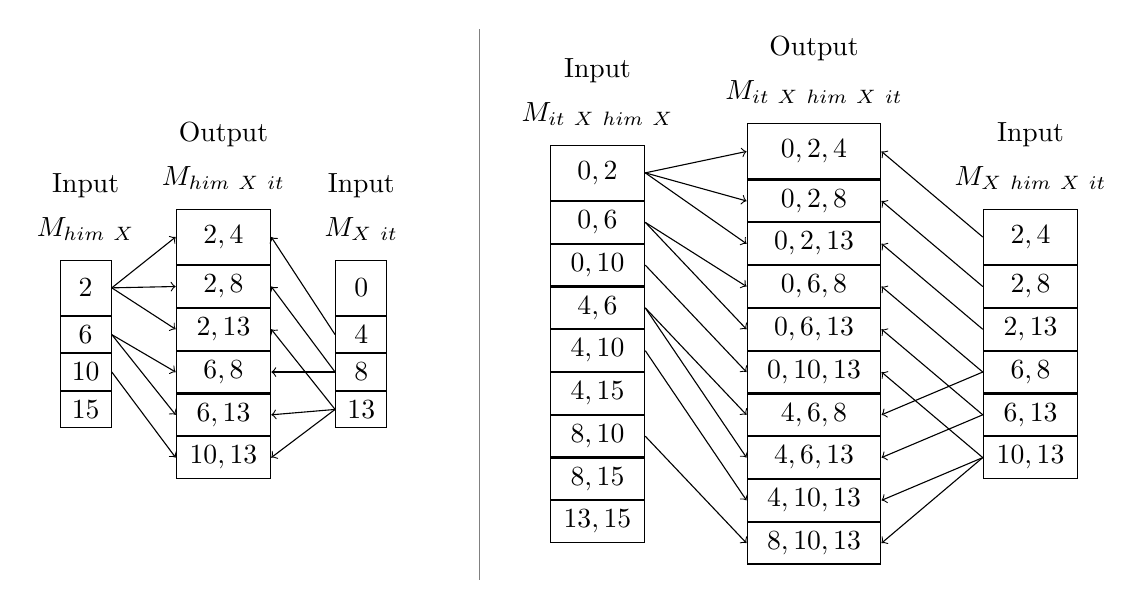
\begin{tikzpicture}[node distance=2.25cm]
	\matrix (him locations) [nodes={rectangle,draw,minimum width=6.5mm}]{
		\node (index 2)  {2}; \\
		\node (index 6)  {6}; \\
		\node (index 10) {10}; \\
		\node (index 15) {15}; \\
	};


	\matrix (him X it locations) [nodes={rectangle,draw,minimum width=12mm},right of=him locations,node distance=1.75cm]{
		\node (index 2 4)   {$2, 4$}; \\
		\node (index 2 8)   {$2, 8$}; \\
		\node (index 2 13)  {$2, 13$}; \\
		\node (index 6 8)   {$6, 8$}; \\
		\node (index 6 13)  {$6, 13$}; \\
		\node (index 10 13) {$10, 13$}; \\
	};


	\matrix (it locations) [nodes={rectangle,draw,minimum width=6.5mm},right of=him X it locations,node distance=1.75cm]{
		\node (index 0)  {0}; \\
		\node (index 4)  {4}; \\
		\node (index 8)  {8}; \\
		\node (index 13) {13}; \\
	};
	
	\node (him label) [anchor=south] at (him locations.north) {$M_{him~X}$};
	\node (pair label) [anchor=south] at (him X it locations.north) {$M_{him~X~it}$};
	\node (it label) [anchor=south] at (it locations.north) {$M_{X~it}$};
	\node [anchor=south] at (him label.north) {Input};
	\node [anchor=south] at (pair label.north) {Output};
	\node [anchor=south] at  (it label.north) {Input};

	\draw[->] (index 2.east) -- (index 2 4.west);
	\draw[->] (index 2.east) -- (index 2 8.west);
	\draw[->] (index 2.east) -- (index 2 13.west);
	\draw[->] (index 6.east) -- (index 6 8.west);
	\draw[->] (index 6.east) -- (index 6 13.west);
	\draw[->] (index 10.east) -- (index 10 13.west);

	\draw[->] (index 4.west) -- (index 2 4.east);
	\draw[->] (index 8.west) -- (index 2 8.east);
	\draw[->] (index 8.west) -- (index 6 8.east);
	\draw[->] (index 13.west) -- (index 2 13.east);
	\draw[->] (index 13.west) -- (index 6 13.east);
	\draw[->] (index 13.west) -- (index 10 13.east);

	\node (between)[right of=it locations,node distance=1.5cm] {};
	\draw[gray,thin] (between.center) -- +(0cm, 4cm);
	\draw[gray,thin] (between.center) -- +(0cm,-3cm);

	\matrix (it X him locations) [nodes={rectangle,draw,minimum width=12mm},right of=it locations,node distance=3cm]{
		\node (index 0 2)   {$0,2$}; \\
		\node (index 0 6)   {$0,6$}; \\
		\node (index 0 10)   {$0,10$}; \\
		\node (index 4 6)   {$4,6$}; \\
		\node (index 4 10)   {$4,10$}; \\
		\node (index 4 15)   {$4,15$}; \\
		\node (index 8 10)   {$8,10$}; \\
		\node (index 8 15)   {$8,15$}; \\
		\node (index 13 15)  {$13,15$}; \\
	};

	\matrix (it X him X it locations) [nodes={rectangle,draw,minimum width=17mm},right of=it X him locations,node distance=2.75cm]{
		\node (index 0 2 4)  {$0,2,4$}; \\
		\node (index 0 2 8)  {$0,2,8$}; \\
		\node (index 0 2 13)  {$0,2,13$}; \\
		\node (index 0 6 8)  {$0,6,8$}; \\
		\node (index 0 6 13)  {$0,6,13$}; \\
		\node (index 0 10 13)  {$0,10,13$}; \\
		\node (index 4 6 8)  {$4,6,8$}; \\
		\node (index 4 6 13)  {$4,6,13$}; \\
		\node (index 4 10 13)  {$4,10,13$}; \\
		\node (index 8 10 13)  {$8,10,13$}; \\
	};


	\matrix (him X it locations) [nodes={rectangle,draw,minimum width=12mm},right of=it X him X it locations,node distance=2.75cm]{
		\node (index 2 4)   {$2, 4$}; \\
		\node (index 2 8)   {$2, 8$}; \\
		\node (index 2 13)  {$2, 13$}; \\
		\node (index 6 8)   {$6, 8$}; \\
		\node (index 6 13)  {$6, 13$}; \\
		\node (index 10 13) {$10, 13$}; \\
	};

	\node (him label) [anchor=south] at (him X it locations.north) {$M_{X~him~X~it}$};
	\node (pair label) [anchor=south] at (it X him X it locations.north) {$M_{it~X~him~X~it}$};
	\node (it label) [anchor=south] at (it X him locations.north) {$M_{it~X~him~X}$};
	\node [anchor=south] at (him label.north) {Input};
	\node [anchor=south] at (pair label.north) {Output};
	\node [anchor=south] at  (it label.north) {Input};

	\draw[->] (index 0 2.east) -- (index 0 2 4.west);
	\draw[->] (index 0 2.east) -- (index 0 2 8.west);
	\draw[->] (index 0 2.east) -- (index 0 2 13.west);
	\draw[->] (index 0 6.east) -- (index 0 6 8.west);
	\draw[->] (index 0 6.east) -- (index 0 6 13.west);
	\draw[->] (index 0 10.east) -- (index 0 10 13.west);
	\draw[->] (index 4 6.east) --  (index 4 6 8.west);
	\draw[->] (index 4 6.east) --  (index 4 6 13.west);
	\draw[->] (index 4 10.east) -- (index 4 10 13.west);
	\draw[->] (index 8 10.east) -- (index 8 10 13.west);

	\draw[->] (index 2 4.west) -- (index 0 2 4.east);
	\draw[->] (index 2 8.west) -- (index 0 2 8.east);
	\draw[->] (index 2 13.west) -- (index 0 2 13.east);
	\draw[->] (index 6 8.west) --  (index 0 6 8.east);
	\draw[->] (index 6 13.west) -- (index 0 6 13.east);
	\draw[->] (index 6 8.west) --  (index 4 6 8.east);
	\draw[->] (index 6 13.west) -- (index 4 6 13.east);
	\draw[->] (index 10 13.west) -- (index 0 10 13.east);
	\draw[->] (index 10 13.west) -- (index 4 10 13.east);
	\draw[->] (index 10 13.west) -- (index 8 10 13.east);

\end{tikzpicture}






	\end{center}}
	\figpostamble
	\caption[\queryfunc\ examples.]{\queryfunc\ examples showing all input and output
	 	sets in sorted order and identifying the pair of input
		matchings that contribute to each output matching.}
	\label{fig:merge-example}
\end{figure}


\noindent Let's turn to the design of the \queryfunc\ algorithm that finds these partners.
First, consider a simple algorithm \intersectfunc\ on two sorted sets $L_1$ and $L_2$.
It computes sorted output set $L_{1 \cap 2}$ containing all
elements common to both $L_1$ and $L_2$ by iteratively comparing the
their topmost elements.  At each iteration, the lesser of the 
two elements is popped from its respective set and discarded.  If the elements
are equal, both are popped and a copy is appended to $L_{1 \cap 2}$.
The complexity of \intersectfunc\ is linear, $O(|L_1| + |L_2|)$.

We can implement \queryfunc\ using
roughly the same logic as \intersectfunc\ if 
$M_{a\alpha}$ and $M_{\alpha{}b}$ are sorted.
For the moment, we will simply assume sortedness.  Later, we will
show how this property is maintained.
The comparison operators that we have defined for partners will
stand in for the comparisons in \intersectfunc.
However, we still need to address a few subtleties.
An important difference between \queryfunc\ and \intersectfunc\
should be apparent from an inspection of example inputs and
outputs (Figure~\ref{fig:merge-example}).  It is possible 
that a matching from either input list partners with multiple
matchings from the other set.  We don't want to pop an item
from the set until we are certain that we have found all of
its partners.

\figpreamble
\begin{figure}
	\figfontsize{
	\begin{center}
		\begin{tikzpicture}[node distance=2.25cm]
	\matrix (him locations) [nodes={rectangle,draw,minimum width=6.5mm}]{
		\node (index 2)  {2}; \\
		\node [fill=lightgray](index 6)  {6}; \\
		\node (index 10) {10}; \\
		\node (index 15) {15}; \\
	};


	\matrix (him X it locations) [nodes={rectangle,draw,minimum width=12mm},right of=him locations,node distance=1.75cm]{
		\node (index 2 4)   {$2, 4$}; \\
		\node (index 2 8)   {$2, 8$}; \\
		\node (index 2 13)  {$2, 13$}; \\
		\node [fill=lightgray](index 6 8)   {$6, 8$}; \\
		\node [fill=lightgray](index 6 13)  {$6, 13$}; \\
		\node (index 10 13) {$10, 13$}; \\
	};


	\matrix (it locations) [nodes={rectangle,draw,minimum width=6.5mm},right of=him X it locations,node distance=1.75cm]{
		\node (index 0)  {0}; \\
		\node (index 4)  {4}; \\
		\node [fill=lightgray](index 8)  {8}; \\
		\node [fill=lightgray](index 13) {13}; \\
	};

	\draw[snake=brace,raise snake=1mm] (index 0.north east) -- (index 4.south east);
	\draw[snake=brace,raise snake=1mm] (index 8.north east) -- (index 13.south east);
%	\node [anchor=west,right=2mm] at (index 0.south east) {$(6) \ddot{>} q_{X~it}$};
%	\node [anchor=west,right=2mm] at (index 8.south east) {$(6) \ddot{=} q_{X~it}$};
	\node [anchor=west,right=2mm] at (index 0.south east) {$\ddot{>}$};
	\node (equal)[anchor=west,right=2mm] at (index 8.south east) {$\ddot{=}$};
	\node [anchor=north,below=4mm] at (equal.south) {$\ddot{<}$ is $\emptyset$};

	\node (him label) [anchor=south] at (him locations.north) {$M_{him~X}$};
	\node (pair label) [anchor=south] at (him X it locations.north) {$M_{him~X~it}$};
	\node (it label) [anchor=south] at (it locations.north) {$M_{X~it}$};
	\node [anchor=south] at (him label.north) {Input};
	\node [anchor=south] at (pair label.north) {Output};
	\node [anchor=south] at  (it label.north) {Input};

	\fill[lightgray] 
		(index 6.south east) --
		(index 6.north east) --
		(index 6 8.north west) --
		(index 6 13.south west) -- cycle;

	\fill[lightgray] 
		(index 6 13.south east) --
		(index 6 8.north east) --
		(index 8.north west) --
		(index 13.south west) -- cycle;
		

	\draw[->] (index 2.east) -- (index 2 4.west);
	\draw[->] (index 2.east) -- (index 2 8.west);
	\draw[->] (index 2.east) -- (index 2 13.west);
	\draw[->] (index 6.east) -- (index 6 8.west);
	\draw[->] (index 6.east) -- (index 6 13.west);
	\draw[->] (index 10.east) -- (index 10 13.west);

	\draw[->] (index 4.west) -- (index 2 4.east);
	\draw[->] (index 8.west) -- (index 2 8.east);
	\draw[->] (index 8.west) -- (index 6 8.east);
	\draw[->] (index 13.west) -- (index 2 13.east);
	\draw[->] (index 13.west) -- (index 6 13.east);
	\draw[->] (index 13.west) -- (index 10 13.east);


	\node (between)[right of=it locations,node distance=1.5cm] {};
	\draw[gray,thin] (between.center) -- +(0cm, 4cm);
	\draw[gray,thin] (between.center) -- +(0cm,-3cm);

	\matrix (it X him locations) [nodes={rectangle,draw,minimum width=12mm},right of=it locations,node distance=3cm]{
		\node (index 0 2)   {$0,2$}; \\
		\node (index 0 6)   {$0,6$}; \\
		\node (index 0 10)   {$0,10$}; \\
		\node [fill=lightgray](index 4 6)   {$4,6$}; \\
		\node (index 4 10)   {$4,10$}; \\
		\node (index 4 15)   {$4,15$}; \\
		\node (index 8 10)   {$8,10$}; \\
		\node (index 8 15)   {$8,15$}; \\
		\node (index 13 15)  {$13,15$}; \\
	};

	\matrix (it X him X it locations) [nodes={rectangle,draw,minimum width=17mm},right of=it X him locations,node distance=2.75cm]{
		\node (index 0 2 4)  {$0,2,4$}; \\
		\node (index 0 2 8)  {$0,2,8$}; \\
		\node (index 0 2 13)  {$0,2,13$}; \\
		\node (index 0 6 8)  {$0,6,8$}; \\
		\node (index 0 6 13)  {$0,6,13$}; \\
		\node (index 0 10 13)  {$0,10,13$}; \\
		\node [fill=lightgray](index 4 6 8)  {$4,6,8$}; \\
		\node [fill=lightgray](index 4 6 13)  {$4,6,13$}; \\
		\node (index 4 10 13)  {$4,10,13$}; \\
		\node (index 8 10 13)  {$8,10,13$}; \\
	};


	\matrix (him X it locations) [nodes={rectangle,draw,minimum width=12mm},right of=it X him X it locations,node distance=2.75cm]{
		\node (index 2 4)   {$2, 4$}; \\
		\node (index 2 8)   {$2, 8$}; \\
		\node (index 2 13)  {$2, 13$}; \\
		\node [fill=lightgray](index 6 8)   {$6, 8$}; \\
		\node [fill=lightgray](index 6 13)  {$6, 13$}; \\
		\node (index 10 13) {$10, 13$}; \\
	};

	\draw[snake=brace,raise snake=1mm] (index 2 4.north east) -- (index 2 13.south east);
	\draw[snake=brace,raise snake=1mm] (index 6 8.north east) -- (index 6 13.south east);
	\draw[snake=brace,raise snake=1mm] (index 10 13.north east) -- (index 10 13.south east);
%	\node [anchor=west,right=2mm] at (index 2 8.east) {$(4,6) \ddot{>} q_{X~him~X~it}$};
%	\node [anchor=west,right=2mm] at (index 6 8.south east) {$(4,6) \ddot{=} q_{X~him~X~it}$};
%	\node [anchor=west,right=2mm] at (index 10 13.east) {$(4,6) \ddot{<} q_{X~him~X~it}$};
	\node [anchor=west,right=2mm] at (index 2 8.east) {$\ddot{>}$};
	\node [anchor=west,right=2mm] at (index 6 8.south east) {$\ddot{=}$};
	\node [anchor=west,right=2mm] at (index 10 13.east) {$\ddot{<}$};


	\node (him label) [anchor=south] at (him X it locations.north) {$M_{X~him~X~it}$};
	\node (pair label) [anchor=south] at (it X him X it locations.north) {$M_{it~X~him~X~it}$};
	\node (it label) [anchor=south] at (it X him locations.north) {$M_{it~X~him~X}$};
	\node [anchor=south] at (him label.north) {Input};
	\node [anchor=south] at (pair label.north) {Output};
	\node [anchor=south] at  (it label.north) {Input};

	\fill[lightgray] 
		(index 4 6.south east) --
		(index 4 6.north east) --
		(index 4 6 8.north west) --
		(index 4 6 13.south west) -- cycle;

	\fill[lightgray] 
		(index 4 6 13.south east) --
		(index 4 6 8.north east) --
		(index 6 8.north west) --
		(index 6 13.south west) -- cycle;


	\draw[->] (index 0 2.east) -- (index 0 2 4.west);
	\draw[->] (index 0 2.east) -- (index 0 2 8.west);
	\draw[->] (index 0 2.east) -- (index 0 2 13.west);
	\draw[->] (index 0 6.east) -- (index 0 6 8.west);
	\draw[->] (index 0 6.east) -- (index 0 6 13.west);
	\draw[->] (index 0 10.east) -- (index 0 10 13.west);
	\draw[->] (index 4 6.east) --  (index 4 6 8.west);
	\draw[->] (index 4 6.east) --  (index 4 6 13.west);
	\draw[->] (index 4 10.east) -- (index 4 10 13.west);
	\draw[->] (index 8 10.east) -- (index 8 10 13.west);

	\draw[->] (index 2 4.west) -- (index 0 2 4.east);
	\draw[->] (index 2 8.west) -- (index 0 2 8.east);
	\draw[->] (index 2 13.west) -- (index 0 2 13.east);
	\draw[->] (index 6 8.west) --  (index 0 6 8.east);
	\draw[->] (index 6 13.west) -- (index 0 6 13.east);
	\draw[->] (index 6 8.west) --  (index 4 6 8.east);
	\draw[->] (index 6 13.west) -- (index 4 6 13.east);
	\draw[->] (index 10 13.west) -- (index 0 10 13.east);
	\draw[->] (index 10 13.west) -- (index 4 10 13.east);
	\draw[->] (index 10 13.west) -- (index 8 10 13.east);

\end{tikzpicture}

	\end{center}}
	\figpostamble
	\caption{Examples showing the division of $M_{\alpha{}b}$
		into regions by $m_{a\alpha} \in M_{a\alpha}$.}
	\label{fig:prefix-region}
\end{figure}

Let's first consider a matching $m_{a\alpha}$ of prefix
pattern $a\alpha$.  Let $m_\alpha = s(m_{a\alpha})$.
Any partner $m_{\alpha{}b}$ must satisfy the constraint
$p(m_{\alpha{}b}) = m_\alpha$.  From the definition of
the prefix matching, we see that if $\alpha = \beta{}c$,
then the only valid value for $m_{\alpha{}b}$ is in 
fact $m_\alpha$.  If $\alpha = \beta{}X$, then $m_\alpha$
completely determines all elements of $m_{\alpha{}b}$ except
for the final one, $m_{\alpha{}b,K_{\alpha{}b}}$.  In either case,
since $M_{\alpha{}b}$ is sorted, all matchings of $\alpha{}b$
meeting the constraint must occur in the same (possibly empty) 
contiguous region of $M_{\alpha{}b}$.  Sortedness further
guarantees that for all elements $m_{\alpha{}b} \in M_{\alpha{}b}$
subsequent to this region,
$m_{a\alpha} \ddot{<} m_{\alpha{}b}$ by definition of the
comparison operators.  It likewise guarantees that for 
all elements $m_{\alpha{}b} \in M_{\alpha{}b}$ prior to this region,
$m_{a\alpha} \ddot{>} m_{\alpha{}b}$.  Therefore, matching
$m_{a\alpha}$ divides $M_{\alpha{}b}$ into three distinct
regions, any of which may be empty (Figure~\ref{fig:prefix-region}).
This means that we can pop
$m_{a\alpha}$ when we encounter the first element 
$m_{\alpha{}b}$ such that $m_{a\alpha} \ddot{<} m_{\alpha{}b}$
or when we reach the end of the set.

\figpreamble
\begin{figure}
	\figfontsize{
	\begin{center}
		\begin{tikzpicture}[node distance=2.25cm]

	\matrix (it X him locations) [nodes={rectangle,draw,minimum width=12mm}]{
		\node (index 0 2)   {$0,2$}; \\
		\node [fill=lightgray](index 0 6)   {$0,6$}; \\
		\node (index 0 10)   {$0,10$}; \\
		\node [fill=lightgray](index 4 6)   {$4,6$}; \\
		\node (index 4 10)   {$4,10$}; \\
		\node (index 4 15)   {$4,15$}; \\
		\node (index 8 10)   {$8,10$}; \\
		\node (index 8 15)   {$8,15$}; \\
		\node (index 13 15)  {$13,15$}; \\
	};

	\node [anchor=east] at (index 0 2.west) {$\ddot{<}$};
	\node [anchor=east] at (index 0 6.west) {$\ddot{=}$};
	\node [anchor=east] at (index 0 10.west) {$\ddot{>}$};
	\node [anchor=east] at (index 4 6.west) {$\ddot{=}$};
	\node [anchor=east] at (index 4 10.west) {$\ddot{>}$};
	\node [anchor=east] at (index 4 15.west) {$\ddot{>}$};
	\node [anchor=east] at (index 8 10.west) {$\ddot{>}$};
	\node [anchor=east] at (index 8 15.west) {$\ddot{>}$};
	\node [anchor=east] at (index 13 15.west) {$\ddot{>}$};

	\matrix (it X him X it locations) [nodes={rectangle,draw,minimum width=17mm},right of=it X him locations,node distance=2.5cm]{
		\node (index 0 2 4)  {$0,2,4$}; \\
		\node (index 0 2 8)  {$0,2,8$}; \\
		\node (index 0 2 13)  {$0,2,13$}; \\
		\node [fill=lightgray](index 0 6 8)  {$0,6,8$}; \\
		\node (index 0 6 13)  {$0,6,13$}; \\
		\node (index 0 10 13)  {$0,10,13$}; \\
		\node [fill=lightgray](index 4 6 8)  {$4,6,8$}; \\
		\node (index 4 6 13)  {$4,6,13$}; \\
		\node (index 4 10 13)  {$4,10,13$}; \\
		\node (index 8 10 13)  {$8,10,13$}; \\
	};


	\matrix (him X it locations) [nodes={rectangle,draw,minimum width=12mm},right of=it X him X it locations,node distance=2.5cm]{
		\node (index 2 4)   {$2, 4$}; \\
		\node (index 2 8)   {$2, 8$}; \\
		\node (index 2 13)  {$2, 13$}; \\
		\node [fill=lightgray](index 6 8)   {$6, 8$}; \\
		\node (index 6 13)  {$6, 13$}; \\
		\node (index 10 13) {$10, 13$}; \\
	};

	\fill[lightgray]
		(index 0 6.south east) --
		(index 0 6.north east) --
		(index 0 6 8.north west) --
		(index 0 6 8.south west) --cycle;

	\fill[lightgray]
		(index 4 6.south east) --
		(index 4 6.north east) --
		(index 4 6 8.north west) --
		(index 4 6 8.south west) --cycle;

	\fill[lightgray]
		(index 0 6 8.south east) --
		(index 0 6 8.north east) --
		(index 6 8.north west) --
		(index 6 8.south west) --cycle;

	\fill[lightgray]
		(index 4 6 8.south east) --
		(index 4 6 8.north east) --
		(index 6 8.north west) --
		(index 6 8.south west) --cycle;



	\node (him label) [anchor=south] at (him X it locations.north) {$M_{him~X~it~X}$};
	\node (pair label) [anchor=south] at (it X him X it locations.north) {$M_{it~X~him~X~it}$};
	\node (it label) [anchor=south] at (it X him locations.north) {$M_{X~it~X~him}$};
	\node [anchor=south] at (him label.north) {Input};
	\node [anchor=south] at (pair label.north) {Output};
	\node [anchor=south] at  (it label.north) {Input};

	\draw[->] (index 0 2.east) -- (index 0 2 4.west);
	\draw[->] (index 0 2.east) -- (index 0 2 8.west);
	\draw[->] (index 0 2.east) -- (index 0 2 13.west);
	\draw[->] (index 0 6.east) -- (index 0 6 8.west);
	\draw[->] (index 0 6.east) -- (index 0 6 13.west);
	\draw[->] (index 0 10.east) -- (index 0 10 13.west);
	\draw[->] (index 4 6.east) --  (index 4 6 8.west);
	\draw[->] (index 4 6.east) --  (index 4 6 13.west);
	\draw[->] (index 4 10.east) -- (index 4 10 13.west);
	\draw[->] (index 8 10.east) -- (index 8 10 13.west);

	\draw[->] (index 2 4.west) -- (index 0 2 4.east);
	\draw[->] (index 2 8.west) -- (index 0 2 8.east);
	\draw[->] (index 2 13.west) -- (index 0 2 13.east);
	\draw[->] (index 6 8.west) --  (index 0 6 8.east);
	\draw[->] (index 6 13.west) -- (index 0 6 13.east);
	\draw[->] (index 6 8.west) --  (index 4 6 8.east);
	\draw[->] (index 6 13.west) -- (index 4 6 13.east);
	\draw[->] (index 10 13.west) -- (index 0 10 13.east);
	\draw[->] (index 10 13.west) -- (index 4 10 13.east);
	\draw[->] (index 10 13.west) -- (index 8 10 13.east);


	\node (separator) [right of=him X it locations,node distance=1.25cm] {}; 
	\draw[gray,thin] (separator.center) -- +(0cm,4cm);
	\draw[gray,thin] (separator.center) -- +(0cm,-3cm);

	\matrix (it X him locations) [nodes={rectangle,draw,minimum width=12mm},right of=him X it locations,node distance=3cm]{
		\node (index 0 2)   {$\colorbox{lightgray}{0},2$}; \\
		\node [fill=lightgray](index 0 6)   {$\colorbox{lightgray}{0},6$}; \\
		\node (index 0 10)   {$\colorbox{lightgray}{0},10$}; \\
		\node [fill=lightgray](index 4 6)   {$\colorbox{lightgray}{4},6$}; \\
		\node (index 4 10)   {$\colorbox{lightgray}{4},10$}; \\
		\node (index 4 15)   {$\colorbox{lightgray}{4},15$}; \\
		\node (index 8 10)   {$8,10$}; \\
		\node (index 8 15)   {$8,15$}; \\
		\node (index 13 15)  {$13,15$}; \\
	};

	\draw[snake=brace,raise snake=1mm] (index 4 15.south west) -- (index 0 2.north west);
	\draw[snake=brace,raise snake=1mm] (index 13 15.south west) -- (index 8 10.north west);
	\node[anchor=east,left=2mm,text width=4mm] at (index 0 10.south west) {$\ddot{<}$, $\ddot{=}$, or $\ddot{>}$};
	\node[anchor=east,left=2mm] at (index 8 15.west) {$\ddot{>}$};

	\matrix (it X him X it locations) [nodes={rectangle,draw,minimum width=17mm},right of=it X him locations,node distance=2.5cm]{
		\node (index 0 2 4)  {$0,2,4$}; \\
		\node (index 0 2 8)  {$0,2,8$}; \\
		\node (index 0 2 13)  {$0,2,13$}; \\
		\node [fill=lightgray](index 0 6 8)  {$0,6,8$}; \\
		\node (index 0 6 13)  {$0,6,13$}; \\
		\node (index 0 10 13)  {$0,10,13$}; \\
		\node [fill=lightgray](index 4 6 8)  {$4,6,8$}; \\
		\node (index 4 6 13)  {$4,6,13$}; \\
		\node (index 4 10 13)  {$4,10,13$}; \\
		\node (index 8 10 13)  {$8,10,13$}; \\
	};


	\matrix (him X it locations) [nodes={rectangle,draw,minimum width=12mm},right of=it X him X it locations,node distance=2.5cm]{
		\node (index 2 4)   {$2, 4$}; \\
		\node (index 2 8)   {$2, 8$}; \\
		\node (index 2 13)  {$2, 13$}; \\
		\node [fill=lightgray](index 6 8)   {$6, 8$}; \\
		\node (index 6 13)  {$6, 13$}; \\
		\node (index 10 13) {$10, 13$}; \\
	};

	\fill[lightgray]
		(index 0 6.south east) --
		(index 0 6.north east) --
		(index 0 6 8.north west) --
		(index 0 6 8.south west) --cycle;

	\fill[lightgray]
		(index 4 6.south east) --
		(index 4 6.north east) --
		(index 4 6 8.north west) --
		(index 4 6 8.south west) --cycle;

	\fill[lightgray]
		(index 0 6 8.south east) --
		(index 0 6 8.north east) --
		(index 6 8.north west) --
		(index 6 8.south west) --cycle;

	\fill[lightgray]
		(index 4 6 8.south east) --
		(index 4 6 8.north east) --
		(index 6 8.north west) --
		(index 6 8.south west) --cycle;

	\node (him label) [anchor=south] at (him X it locations.north) {$M_{X~him~X~it}$};
	\node (pair label) [anchor=south] at (it X him X it locations.north) {$M_{it~X~him~X~it}$};
	\node (it label) [anchor=south] at (it X him locations.north) {$M_{it~X~him~X}$};
	\node [anchor=south] at (him label.north) {Input};
	\node [anchor=south] at (pair label.north) {Output};
	\node [anchor=south] at  (it label.north) {Input};

	\draw[->] (index 0 2.east) -- (index 0 2 4.west);
	\draw[->] (index 0 2.east) -- (index 0 2 8.west);
	\draw[->] (index 0 2.east) -- (index 0 2 13.west);
	\draw[->] (index 0 6.east) -- (index 0 6 8.west);
	\draw[->] (index 0 6.east) -- (index 0 6 13.west);
	\draw[->] (index 0 10.east) -- (index 0 10 13.west);
	\draw[->] (index 4 6.east) --  (index 4 6 8.west);
	\draw[->] (index 4 6.east) --  (index 4 6 13.west);
	\draw[->] (index 4 10.east) -- (index 4 10 13.west);
	\draw[->] (index 8 10.east) -- (index 8 10 13.west);

	\draw[->] (index 2 4.west) -- (index 0 2 4.east);
	\draw[->] (index 2 8.west) -- (index 0 2 8.east);
	\draw[->] (index 2 13.west) -- (index 0 2 13.east);
	\draw[->] (index 6 8.west) --  (index 0 6 8.east);
	\draw[->] (index 6 13.west) -- (index 0 6 13.east);
	\draw[->] (index 6 8.west) --  (index 4 6 8.east);
	\draw[->] (index 6 13.west) -- (index 4 6 13.east);
	\draw[->] (index 10 13.west) -- (index 0 10 13.east);
	\draw[->] (index 10 13.west) -- (index 4 10 13.east);
	\draw[->] (index 10 13.west) -- (index 8 10 13.east);

\end{tikzpicture}

	\end{center}}
	\figpostamble
	\caption[xample showing the relationships of $m_{a\alpha} \in M_{a\alpha}$
		to an element $m_{\alpha{}b}$.]{Example showing the relationships of $m_{a\alpha} \in M_{a\alpha}$ to an element $m_{\alpha{}b}$, and the subsequent delineation of
		$M_{a\alpha}$ into regions by $m_{\alpha{}b}$.}
	\label{fig:suffix-region}
\end{figure}

Now let's consider a matching $m_{\alpha{}b}$ of suffix
pattern $\alpha{}b$.  Let $m_\alpha = p(m_{\alpha{}b})$.
Any partner $m_{a\alpha}$ must satisfy the constraint
$s(m_{a\alpha}) = m_\alpha$.  From the definition of
the suffix matching, we see that if $\alpha = c\beta$,
then there is only one valid value for $m_{a\alpha}$.  In
this case, sortedness ensures that $m_{\alpha{}b}$
divides $M_{a\alpha}$ into three regions, just as we
saw for the prefix matchings.  Matters are different
if $\alpha = X\beta$.  In this case, $m_\alpha$
completely determines all elements of $m_{a\alpha}$
except for the first one, $m_{a\alpha,1}$.  This element
could take several values.  Furthermore, each of these values 
can be the first element of several matchings.  Only one of
these matching will meet our constraint, and thus
the rest won't be partners with $m_{\alpha{}b}$.  As a consequence,
it is possible for partners of $m_{\alpha{}b}$ to be 
interspersed with non-partners (Figure~\ref{fig:suffix-region}).
However, our definitions ensure that there is a contiguous 
range of possible values for $m_{\alpha{}b,1}$.
Sortedness ensures that the set of all matchings 
$m_{a\alpha} \in M_{a\alpha}$ for which $m_{\alpha{}b,1}$ is in this
range must occur in a contiguous region of $M_{a\alpha}$.
Furthermore, our definitions ensure that for any 
value $i$, if $m_{a\alpha} \ddot{>} m_{\alpha{}b}$ for the first occurrence
of a matching $m_{a\alpha}$ such $m_{ab\alpha,1} = i$,
then for all subsequent matchings $m_{a\alpha} \in M_{a\alpha}$,
$m_{a\alpha} \ddot{>} m_{\alpha{}b}$.  An analogous case
occurs for matchings $m_{a\alpha} \in M_{a\alpha}$ such that
$m_{a\alpha} \ddot{<} m_{\alpha{}b}$.  Therefore, $m_{\alpha{}b}$
divide $M_{a\alpha}$ into three regions, each of which may
possibly be empty.  However, it is possible for values in
the central region to have any relationship with $m_{\alpha{}b}$,
and therefore we must check all of them.  We can safely
pop $m_{\alpha{}b}$ when we encounter a matching
$m_{a\alpha}$ such that $m_{a\alpha} \ddot{>} m_{\alpha{}b}$ and
whose first element $m_{a\alpha,1}$ has not been seen before.

\algorithm{The basic \queryfunc\ algorithm}{
	\label{alg:query-intersect}
	\noindent {\bf Function} {\sc Query\_Intersect}

\noindent {\bf Input:} sorted prefix matchings $M_{a\alpha}$ and sorted suffix matchings $M_{\alpha{}b}$
\begin{algorithmic}[1]

	\State $M_{a\alpha{}b} \leftarrow \emptyset$
	\State $I \leftarrow |M_{a\alpha}|$
	\State $J \leftarrow |M_{\alpha{}b}|$
	\State $j \leftarrow 0$
	\State $m_1 \leftarrow -1$
	\For {$i$ from $0$ to $I$}
		\State $m_{a\alpha} \leftarrow M_{a\alpha}[i]$
		\State $m_{\alpha{}b} \leftarrow M_{\alpha{}b}[j]$
		\If {$m_{a\alpha,1} \neq m_1$}
			\While {$m_{a\alpha} \ddot{>} m_{\alpha{}b}$ and $j < J$}
				\State $j \leftarrow j + 1$
				\State $m_{\alpha{}b} \leftarrow M_{\alpha{}b}[j]$
			\EndWhile
			\If {$m_{a\alpha} \ddot{>} m_{\alpha{}b}$ and $j = J$}
				\State Break
			\EndIf
		\EndIf
		\State $k \leftarrow j$
		\While {not $m_{a\alpha} \ddot{<} m_{\alpha{}b}$}
			\If {$m_{a\alpha} \ddot{=} m_{\alpha{}b}$}
				\State Append $m_{a\alpha} \bowtie m_{\alpha{}b}$ to $M_{a\alpha{}b}$
			\EndIf
			\If {$k = J$}
				\State Break
			\Else
				\State $k \leftarrow k + 1$
				\State $m_{\alpha{}b} \leftarrow M_{\alpha{}b}[k]$
			\EndIf
		\EndWhile
	\EndFor
	\State \Return {$M_{a\alpha{}b}$}
\end{algorithmic}

}


The full \queryfunc\ algorithm (Listing~\ref{alg:query-intersect}) is non-destructive -- we
advance a pointer rather than popping matchings from each set.  Its operation is
similar to \intersectfunc, though we take a different approach to popping matchings
from the stack.  For each matching $m_{a\alpha} \in M_{a\alpha}$, we scan 
downwards from the current top of $M_{\alpha{}b}$, joining $m_{a\alpha}$ with any
partners as we find them, until we encounter $m_{\alpha{}b}$ such that
$m_{a\alpha} \ddot{<} m_{\alpha{}b}$.  We then pop $m_{a\alpha}$.  Elements
$m_{\alpha{}b} \in M_{\alpha{}b}$ are popped whenever we uncover a new
top matching $m_{a\alpha} \in M_{a\alpha}$ such that 
$m_{a\alpha} \ddot{>} m_{\alpha{}b}$ and whose first element $m_{a\alpha,1}$
has not been seen before.  

The upper bound complexity of \queryfunc\ is $O(|M_{a\alpha}| \times |M_{\alpha{}b}|)$.
However, most matchings can be popped from their respective sets after a single
comparison, so the average case complexity is closer to 
$O(|M_{a\alpha}| + |M_{\alpha{}b}|)$.  Both upper bound and average complexity are
identical to that of the baseline algorithm.  As we've seen, though, our
enumeration algorithm enables us to call it much less frequently using
smaller input sets than in the baseline.

We assume that $M_{a\alpha}$ is
sorted, and we process its matchings in order.  Furthermore, for any
$m_{a\alpha} \in M_{a\alpha}$, recall that its partners can only differ
on their last element, and that these are encountered in sorted order.
Therefore, the output of \queryfunc\ is sorted.  This means that
if we call \queryfunc\ using input sets that resulted from a previous
invocation of \queryfunc, they will already be sorted.
We must still ensure sortedness in the base case, which occurs when 
either prefix $a\alpha$ or suffix $\alpha{}b$ contains a single
contiguous pattern.  In this case, the set $M_{a\alpha}$ or
$M_{\alpha{}b}$ is the result of a search in the suffix array.
As we saw earlier, this set is not returned in sorted
order.  To solve this, we explicitly sort the occurrences by inserting
them into a stratified tree \citep{emde-boas:1977:mst} and
reading the sorted sequence from the tree.  Sort
time is $O(|M_\alpha| \log\log |T|)$ for a pattern $\alpha$.
This is superlinear, but we need to sort only
once, since we cache the result at the corresponding
prefix tree node.  Since we expect to query the text for many patterns containing this
subpattern, the cost is amortized over all computations.
Overall, this means that ensuring sortedness
adds computational expense to our algorithm.  
This will be counterbalanced by additional strategies that exploit
sortedness, introduced in the next sections.



\subsubsection{Precomputation of Inverted Indices for Frequent Subpatterns}\label{sec:inverted-indices}

Sorting the matchings of a contiguous pattern $w$
adds an $O(|M_w| \log\log |T|)$ term to 
query complexity.  This is fine for infrequent patterns. However,
if $|M_w|$ is large, this may be quite expensive.

We can circumvent this problem by precomputing an 
{\em inverted index} \citep{Zobel:2006:csur}.
This is simply the list $|M_w|$ in sorted order.  
It can be computed in one pass over the data.  The memory consumption
of inverted indices for all $n$-grams up to some maximum
$n$ requires $n |T|$ space, so using this strategy for all
$n$-grams is infeasible.
Instead we precompute the inverted index only for the most
frequent $n$-grams.\footnote{We identify the most frequent patterns
in a single traversal over the {\em longest common prefix (LCP) array},
an auxiliary data structure of the suffix array 
\citep{Manber:1993:sicomp}.  We only need the LCP array for this purpose, 
so we compute it once offline using a fast algorithm due to 
\citet{Kasai:2001:cpm}.} For less frequent $n$-grams, we continue to 
generate the index on the fly using stratified trees as before.

\subsection{Faster Pattern Matching for Individual Query Patterns}
\label{sec:efficient-lookup}

The complexity of the comparison step in 
both the baseline algorithm and our merge algorithm is
linear in the number of occurrences of each subpattern.
Therefore, the main improvement we have introduced so far is
reduction in the number of unnecessary lookups.  The cost
of pattern matching for a single query pattern is mostly unchanged, and as
we have seen, it can be very expensive whenever
the query pattern contains a frequent subpattern.
However, there is a silver lining.
Recall that patterns follow a Zipf distribution 
(Figure~\ref{fig:ngram-histogram}), so
the number of pattern types that cause the problem
is quite small.  The vast majority of patterns
are rare.  Therefore, our solution focuses on patterns 
with one or more frequent subpatterns.  
To simplify matters, we focus on the intermediate computation
for pattern $w_1 X ... X w_k$.  This requires us
to compute the collocation of subpatterns $w_1 X ... X w_{k-1}$ 
and $w_{k}$.  There are three cases.

\begin{itemize}
	\item If both patterns are rare, we use the \queryfunc\ algorithm (\textsection\ref{sec:collocation-algorithm}).

	\item If one pattern is frequent and the other is rare, we
	use an algorithm whose complexity depends mainly on the 
	frequency of the rare pattern (see \textsection\ref{sec:double-binary}, below).  
	It can also be used for pairs of rare patterns when one 
	pattern is much rarer than the other.

	\item If both patterns are frequent, we resort to a precomputed
	intersection (see \textsection\ref{sec:precomputation}, below).  We are
	not aware of any algorithms to substantially improve the efficiency
	of this computation at runtime, but the result can be precomputed
	in a single pass over the text.\footnote{We combine this with the
	precomputation of inverted indices (\textsection\ref{sec:inverted-indices}).}
\end{itemize}

\subsubsection{Fast Intersection via Double Binary Search}\label{sec:double-binary}

For collocations of frequent and rare patterns, 
we use a fast set intersection method for sorted
sets called {\em double binary search}
\citep{Baeza-Yates:2004:cpm}.  Suppose that we
wish to intersect a sorted set $Q$ with a much larger
sorted set $Q'$.  Note that we can compute this 
intersection efficiently by performing a binary 
search in $Q'$ for each element of $Q$.  The
complexity is $\Theta(|Q| \log |Q'|)$, which
is better than the \intersectfunc\ algorithm complexity
of $O(|Q| + |Q'|)$ if $Q \ll Q'$.  Note
that this is a tight bound.

Double binary search takes this idea a step further.  
It performs a binary search in $Q'$ for the median
element of $Q$.  Whether or not the element is found,
the result divides both sets into two pairs of smaller sets that
can be processed recursively.  In many cases, one of the
recursive inputs will be empty, and we don't need to
do any work at all.  This results in a loose
bound on complexity, $O(|Q| \log |Q'|)$, and the
average case is often much better than this
\citep{Baeza-Yates:2004:cpm,baeza-yates:2005:spire}.
We can modify the algorithm to compute collocation rather 
than intersection, just as we did for the merge
algorithm (\textsection\ref{sec:collocation-algorithm}).

If $|Q| \log |Q'| < |Q| + |Q'|$ then the performance
is guaranteed to be sublinear in $|Q| + |Q'|$.  Because the 
bound is loose, it is often sublinear
even if $|Q| \log |Q'|$ is somewhat larger than $|Q| + |Q'|$.
In our implementation we simply
check for the condition  $\lambda |Q| \log |Q'| < |Q| + |Q'|$ to decide
whether we should use double binary search or the merge algorithm.
This check is applied in the recursive cases as well as for the 
initial inputs.  The variable $\lambda$ can be adjusted
for speed.  We explore possible values for it empirically in 
\textsection\ref{sec:algorithmic-timing-results}.

\subsubsection{Precomputation of Collocations}\label{sec:precomputation}

\figpreamble
\begin{figure}
	\figfontsize{
	\begin{center}
		\begin{tikzpicture} [node distance=2.7cm]
	\matrix (sentence) [nodes={text height=10pt}] at (0,0){
	\node (word 0) {it}; & \node (word 1) {makes}; & \node (word 2) {him}; & \node (word 3) {and}; & 
	\node (word 4) {it}; & \node (word 5) {mars}; & \node (word 6) {him}; & \node (word 7) {,}; & 
	\node (word 8) {it}; & \node (word 9) {sets}; & \node (word 10) {him}; & \node (word 11) {on}; & 
	\node (word 12) {and}; & \node (word 13) {it}; & \node (word 14) {takes}; & \node (word 15) {him}; & 
	\node (word 16) {off}; & \node (word 17) {.}; & \node (word 18) {\#};\\
	\node (num 0) {0}; & \node (num 1) {1}; & \node (num 2) {2}; & \node (num 3) {3}; & 
	\node (num 4) {4}; & \node (num 5) {5}; & \node (num 6) {6}; & \node (num 7) {7}; & 
	\node (num 8) {8}; & \node (num 9) {9}; & \node (num 10) {10}; & \node (num 11) {11}; & 
	\node (num 12) {12}; & \node (num 13) {13}; & \node (num 14) {14}; & \node (num 15) {15}; & 
	\node (num 16) {16}; & \node (num 17) {17}; & \node (num 18) {18};\\
	};

	\path (sentence.south) -- +(3.5,-0.75) coordinate (step pos);
	\node (step) [text width=7cm] at (step pos) {\begin{center}Add frequent word and position to queue.\end{center}};

	\path (word 0.north east) -- +(0pt,-35pt) coordinate (pos 0 east);
	\fill[rounded corners,lightgray] (word 0.north west) rectangle (pos 0 east);
	\node (word 0) [text height=10pt] at (word 0.center) {it}; 
	\node (num 0)  [text height=10pt] at (num 0.center) {0};
	
	\path (sentence.south west) -- +(0,-0.75) coordinate (queue loc);
	\node (queue) [anchor=west,right=3pt] at (queue loc) {Queue:};
	\node (queued 0) [draw,text height=10pt,anchor=west] at (queue.east) {it, 0};
	\path (queued 0) -- +(0,1) coordinate (queued 0 north);

	\draw[->] (num 0.south) ..controls +(0,-0.5) and (queued 0 north) .. (queued 0.north);

	\path (sentence.south west) -- +(0,-1.25) coordinate (separator west);
	\path (sentence.south east) -- +(0,-1.25) coordinate (separator east);
	\draw[thin,gray] (separator west) -- (separator east);

	\matrix (sentence) [nodes={text height=10pt},below of=sentence]{
	\node (word 0) {it}; & \node (word 1) {makes}; & \node (word 2) {him}; & \node (word 3) {and}; & 
	\node (word 4) {it}; & \node (word 5) {mars}; & \node (word 6) {him}; & \node (word 7) {,}; & 
	\node (word 8) {it}; & \node (word 9) {sets}; & \node (word 10) {him}; & \node (word 11) {on}; & 
	\node (word 12) {and}; & \node (word 13) {it}; & \node (word 14) {takes}; & \node (word 15) {him}; & 
	\node (word 16) {off}; & \node (word 17) {.}; & \node (word 18) {\#};\\
	\node (num 0) {0}; & \node (num 1) {1}; & \node (num 2) {2}; & \node (num 3) {3}; & 
	\node (num 4) {4}; & \node (num 5) {5}; & \node (num 6) {6}; & \node (num 7) {7}; & 
	\node (num 8) {8}; & \node (num 9) {9}; & \node (num 10) {10}; & \node (num 11) {11}; & 
	\node (num 12) {12}; & \node (num 13) {13}; & \node (num 14) {14}; & \node (num 15) {15}; & 
	\node (num 16) {16}; & \node (num 17) {17}; & \node (num 18) {18};\\
	};

	\path (sentence.south) -- +(3.5,-0.75) coordinate (step pos);
	\node (step) [text width=7cm] at (step pos) {\begin{center}Advance pointer, skipping infrequent words.\end{center}};

	\path (word 1.north east) -- +(0pt,-35pt) coordinate (pos 1 east);
	\fill[rounded corners,lightgray] (word 1.north west) rectangle (pos 1 east);
	\node (word 1) [text height=10pt] at (word 1.center) {makes}; 
	\node (num 1)  [text height=10pt] at (num 1.center) {1};
	
	\path (sentence.south west) -- +(0,-0.75) coordinate (queue loc);
	\node (queue) [anchor=west,right=3pt] at (queue loc) {Queue:};
	\node (queued 0) [draw,text height=10pt,anchor=west] at (queue.east) {it, 0};
	%\path (queued 0) -- +(0,1) coordinate (queued 0 north);
    %
	%\draw[->] (num 0.south) ..controls +(0,-0.5) and (queued 0 north) .. (queued 0.north);

	\path (sentence.south west) -- +(0,-1.25) coordinate (separator west);
	\path (sentence.south east) -- +(0,-1.25) coordinate (separator east);
	\draw[thin,gray] (separator west) -- (separator east);
	
	\matrix (sentence) [nodes={text height=10pt},below of=sentence]{
	\node (word 0) {it}; & \node (word 1) {makes}; & \node (word 2) {him}; & \node (word 3) {and}; & 
	\node (word 4) {it}; & \node (word 5) {mars}; & \node (word 6) {him}; & \node (word 7) {,}; & 
	\node (word 8) {it}; & \node (word 9) {sets}; & \node (word 10) {him}; & \node (word 11) {on}; & 
	\node (word 12) {and}; & \node (word 13) {it}; & \node (word 14) {takes}; & \node (word 15) {him}; & 
	\node (word 16) {off}; & \node (word 17) {.}; & \node (word 18) {\#};\\
	\node (num 0) {0}; & \node (num 1) {1}; & \node (num 2) {2}; & \node (num 3) {3}; & 
	\node (num 4) {4}; & \node (num 5) {5}; & \node (num 6) {6}; & \node (num 7) {7}; & 
	\node (num 8) {8}; & \node (num 9) {9}; & \node (num 10) {10}; & \node (num 11) {11}; & 
	\node (num 12) {12}; & \node (num 13) {13}; & \node (num 14) {14}; & \node (num 15) {15}; & 
	\node (num 16) {16}; & \node (num 17) {17}; & \node (num 18) {18};\\
	};

	\path (sentence.south) -- +(3.5,-0.75) coordinate (step pos);
	\node (step) [text width=7cm] at (step pos) {\begin{center}Iterate through all words.\end{center}};

	\path (word 2.north east) -- +(0pt,-35pt) coordinate (pos 2 east);
	\fill[rounded corners,lightgray] (word 2.north west) rectangle (pos 2 east);
	\node (word 2) [text height=10pt] at (word 2.center) {him}; 
	\node (num 2)  [text height=10pt] at (num 2.center) {2};
	
	\path (sentence.south west) -- +(0,-0.75) coordinate (queue loc);
	\node (queue) [anchor=west,right=3pt] at (queue loc) {Queue:};
	\node (queued 0) [draw,text height=10pt,anchor=west] at (queue.east) {it, 0};
	\node (queued 2) [draw,text height=10pt,anchor=west] at (queued 0.east) {him, 2};
	\path (queued 2) -- +(0,1) coordinate (queued 2 north);
    
	\draw[->] (num 2.south) ..controls +(0,-0.5) and (queued 2 north) .. (queued 2.north);

	\path (sentence.south west) -- +(0,-1.25) coordinate (separator west);
	\path (sentence.south east) -- +(0,-1.25) coordinate (separator east);
	\draw[thin,gray] (separator west) -- (separator east);

	\node [below of=sentence] {...};

	\path (sentence.south west) -- +(0,-2.5) coordinate (separator west);
	\path (sentence.south east) -- +(0,-2.5) coordinate (separator east);
	\draw[thin,gray] (separator west) -- (separator east);

	\matrix (sentence) [nodes={text height=10pt},below of=sentence,node distance=4.6cm]{
	\node (word 0) {it}; & \node (word 1) {makes}; & \node (word 2) {him}; & \node (word 3) {and}; & 
	\node (word 4) {it}; & \node (word 5) {mars}; & \node (word 6) {him}; & \node (word 7) {,}; & 
	\node (word 8) {it}; & \node (word 9) {sets}; & \node (word 10) {him}; & \node (word 11) {on}; & 
	\node (word 12) {and}; & \node (word 13) {it}; & \node (word 14) {takes}; & \node (word 15) {him}; & 
	\node (word 16) {off}; & \node (word 17) {.}; & \node (word 18) {\#};\\
	\node (num 0) {0}; & \node (num 1) {1}; & \node (num 2) {2}; & \node (num 3) {3}; & 
	\node (num 4) {4}; & \node (num 5) {5}; & \node (num 6) {6}; & \node (num 7) {7}; & 
	\node (num 8) {8}; & \node (num 9) {9}; & \node (num 10) {10}; & \node (num 11) {11}; & 
	\node (num 12) {12}; & \node (num 13) {13}; & \node (num 14) {14}; & \node (num 15) {15}; & 
	\node (num 16) {16}; & \node (num 17) {17}; & \node (num 18) {18};\\
	};

	\path (sentence.south) -- +(3.5,-1) coordinate (step pos);
	\node (step) [text width=6cm] at (step pos) {\begin{center}Pop the first item from queue when its distance to current word reaches the maximum pattern length.\end{center}};

	\path (word 9.north east) -- +(0pt,-35pt) coordinate (pos 9 east);
	\fill[rounded corners,lightgray] (word 9.north west) rectangle (pos 9 east);
	\node (word 9) [text height=10pt] at (word 9.center) {sets}; 
	\node (num 9)  [text height=10pt] at (num 9.center) {9};
	
	\path (sentence.south west) -- +(0,-0.75) coordinate (queue loc);
	\node (queue) [anchor=west,right=3pt] at (queue loc) {Queue:};
	\node (queued 0) [lightgray,fill=lightgray,text height=10pt,anchor=west] at (queue.east) {it, 0};
	\node (queued 2) [draw,text height=10pt,anchor=west,right=3mm] at (queued 0.east) {him, 2};
	\node (queued 4) [draw,text height=10pt,anchor=west] at (queued 2.east) {it, 4};
	\node (queued 6) [draw,text height=10pt,anchor=west] at (queued 4.east) {him, 6};
	\node (queued 8) [draw,text height=10pt,anchor=west] at (queued 6.east) {it, 8};
	
	\node (queued 0 popped) [draw,text height=10pt,anchor=west,below of=queued 0,node distance=1.2cm] {it, 0};

	\draw[->] (queued 0.south) -- (queued 0 popped.north);
	\draw[snake=brace,segment amplitude=2mm] (word 0.north west) -- (word 9.north east) node [anchor=south,pos=0.5,above=2mm] {$\maxphrasespan = 10$};

	\path (sentence.south west) -- +(0,-3.5) coordinate (it X him loc);
	\node (it X him) [anchor=west,right=6mm] at (it X him loc) {it $X$ him:};
	\node (it X him 1) [draw,text height=10pt,anchor=west] at (it X him.east) {$0, 2$};
	\node (it X him 2) [draw,text height=10pt,anchor=west] at (it X him 1.east) {$0, 6$};

	\node (it X it) [anchor=west,right=5mm] at (it X him 2.east) {it $X$ it:};
	\node (it X it 1) [draw,text height=10pt,anchor=west] at (it X it.east) {$0, 4$};
	\node (it X it 2) [draw,text height=10pt,anchor=west] at (it X it 1.east) {$0, 8$};
	
	\path (it X him 1.north) -- +(0,1) coordinate (it X him 1 north);
	\path (it X him 2.north) -- +(0,1) coordinate (it X him 2 north);
	\path (it X it 1.north) -- +(0,1) coordinate (it X it 1 north);
	\path (it X it 2.north) -- +(0,1) coordinate (it X it 2 north);
	
	\draw[->] (queued 2.south) ..controls +(0,-1) and (it X him 1 north) .. (it X him 1.north);
	\draw[->] (queued 6.south) ..controls +(0,-1) and (it X him 2 north) .. (it X him 2.north);
	\draw[->] (queued 4.south) ..controls +(0,-1) and (it X it 1 north) .. (it X it 1.north);
	\draw[->] (queued 8.south) ..controls +(0,-1) and (it X it 2 north) .. (it X it 2.north);
	
	\draw[->] (queued 0 popped) ..controls +(0.5,0) and (it X him 1 north) .. (it X him 1.north);
	\draw[->] (queued 0 popped) ..controls +(1,0) and (it X him 2 north) .. (it X him 2.north);
	\draw[->] (queued 0 popped) ..controls +(2,0) and (it X it 1 north) .. (it X it 1.north);
	\draw[->] (queued 0 popped) ..controls +(3,0) and (it X it 2 north) .. (it X it 2.north);

	\path (sentence.south) -- +(3.5,-3.5) coordinate (step pos);
	\node (step) [text width=6cm] at (step pos) {\begin{center}Combine the popped item with each remaining item in the queue, and record the resulting pattern locations.\end{center}};

\end{tikzpicture}

	\end{center}}
	\figpostamble
	\caption{Illustration of the precomputation algorithm.}
	\label{fig:precomputation-algorithm}
\end{figure}

Double binary search only helps if one subpattern is infrequent.
If both subpatterns are frequent, there is no clever algorithm
to efficiently compute their collocation at runtime.  Therefore, we
precompute these expensive collocations
in a single pass over the text.  As input, our algorithm requires the 
identities of the $k$ most frequent contiguous patterns.~
We then iterate over the corpus.  Whenever a pattern from the 
list is seen, we push a tuple consisting of its identity and 
current location onto a queue.  Whenever 
the oldest item on the queue falls on the edge of the 
maximum span window with respect to the current 
position, we pop it from the queue and compute its
collocation with all other items in the queue (subject to any gap
length constraints) .  We repeat this step for every item 
that falls outside the window.  At the end of each
sentence, we compute collocations for any remaining
items in the queue and then empty it.  The algorithm is
illustrated in Figure~\ref{fig:precomputation-algorithm}.

Our precomputation includes the most frequent $n$-gram
subpatterns.  Most of these are unigrams, though
we found $5$-grams among the $1000$ most
frequent patterns.  We precompute the locations of
source phrase $uXv$ for any pair $u$ and $v$ that both
appear on this list.  There is also a small number of
patterns $uXv$ that are very frequent.
We cannot easily obtain a list of these in advance, but
we observe that they always consist of a pair $u$ and $v$ of patterns
from near the top of the frequency list.  Therefore
we also precompute the locations of patterns $uXvXw$
in which both $u$ and $v$ are among these super-frequent
patterns (all unigrams), treating this as the collocation of the 
frequent pattern $uXv$ and frequent pattern $w$.  We
also compute the analogous case for $uXvXw$ when 
$v$ and $w$ are super-frequent.

\subsubsection{Putting it all Together: The Root \queryfunc\ algorithm}

We've described several algorithms for pattern matching on text,
including suffix array lookup for contiguous patterns 
(\textsection\ref{sec:suffix_arrays}) and multiple
algorithms for discontiguous queries including the \queryfunc\ algorithm
(\textsection\ref{sec:collocation-algorithm}),
double binary search (\textsection\ref{sec:double-binary}), and cache retrieval
(\textsection\ref{sec:precomputation}).  To make clear when each
of these algorithms is called, we include here the root \queryfunc\
algorithm that dispatches to the appropriate algorithm for each case
(Listing~\ref{alg:query-main}).  This
is the only \queryfunc\ called for all phrase queries from the prefix tree
algorithm (Listing~\ref{alg:prefix-tree}).

\algorithm{The root \queryfunc\ algorithm}{
	\label{alg:query-main}
	\noindent {\bf Function} {\sc Query\_Root}

\noindent {\bf Input:} pattern $a\alpha{}b$; one of the following: suffix array indices low $\ell_{a\alpha}$ and high $h_{a\alpha}$ if $\alpha=uX$, sorted prefix matchings $M_{a\alpha}$ otherwise; suffix array indices low $\ell_{\alpha{}b}$ and high $h_{\alpha{}b}$ if $\alpha=Xu$, sorted prefix matchings $M_{\alpha{}b}$ otherwise.

\begin{algorithmic}[1]

	\If {$\alpha = u$} \Comment {$\alpha$ is a contiguous pattern}
		\State \Return {\Call{Suffix-Array-Lookup}{$SA_F, a\alpha{}b, \ell_{a\alpha}, h_{a\alpha}$}}
	\Else \Comment {$\alpha$ is a discontiguous pattern}
		\If {$\alpha=uX$} \Comment {prefix is a contiguous pattern}
			\State $M_{a\alpha} \leftarrow$  \Call{Sort\_Matchings}{$a\alpha, \ell_{a\alpha}, h_{a\alpha}$}
		\EndIf
		\If {$\alpha=Xu$} \Comment {suffix is a contiguous pattern}
			\State $M_{\alpha{}b} \leftarrow$ \Call{Sort\_Matchings}{$\alpha{}b, \ell_{\alpha{}b}, h_{\alpha{}b}$}
		\EndIf
		\If {$M_{a\alpha{}b}$ has been precomputed}
			\State Retrieve $M_{a\alpha{}b}$ from cache of precomputations
		\Else
			\If {$|M_{a\alpha}| < |M_{\alpha{}b}|$ and $\lambda |M_{a\alpha}| \log |M_{\alpha{}b}| < |M_{a\alpha}| + |M_{\alpha{}b}|$}
				\State $M_{a\alpha{}b} \leftarrow $ \Call{Query\_Double\_Binary}{$M_{a\alpha}, M_{\alpha{}b}$}
			\ElsIf {$|M_{\alpha{}b}| < |M_{a\alpha}|$ and $\lambda |M_{\alpha{}b}| \log |M_{a\alpha}| < |M_{\alpha{}b}| + |M_{a\alpha}|$}
				\State $M_{a\alpha{}b} \leftarrow $ \Call{Query\_Double\_Binary}{$M_{a\alpha}, M_{\alpha{}b}$}
			\Else
				\State $M_{a\alpha{}b} \leftarrow $ \Call{Query\_Intersect}{$M_{a\alpha}, M_{\alpha{}b}$}
			\EndIf
		\EndIf
		\State \Return $M_{a\alpha{}b}$
	\EndIf
\end{algorithmic}

~

\noindent {\bf Function} {\sc Sort\_Matchings}

\noindent {\bf Input:} pattern $\alpha$, suffix array indices $\ell$ and $h$
\begin{algorithmic}[1]
	\If {inverted index $M_\alpha$ has been precomputed}
		\State \Return{precomputed $M_\alpha$ from cache}
	\Else
		\State Let $S$ be a stratified tree
		\State $M_\alpha \leftarrow \emptyset$
		\For {$k$ from $\ell$ to $h$}
			\State \Call{Insert}{$SA_F[k], S$}
		\EndFor
		\State $k \leftarrow $ \Call{Next\_Element}{$-1, S$}
		\While {$k \neq -1$}
			\State \Call{Append}{$k, M_\alpha$}
		\EndWhile
		\State \Return{$M_\alpha$}
	\EndIf
\end{algorithmic}

}

\section{Source-Driven Phrase Extraction}\label{sec:hierarchical-extraction}

\figpreamble
\begin{figure}
	\figfontsize{
	\begin{center}
		\begin{tikzpicture}
	\renewcommand\currentex[1]{\extractionex{5}{1, 3, 5}{2, 4}{1/1, 2/3, 3/2, 4/4, 5/5}{#1}}
	\currentex{}
	\node [anchor=south] at (source 3.north) {\fboxsep1pt 1. Find source phrase $f_2 X_{\fbox{\scriptsize 1}} f_4$.};
	\path (target 1.south west) -- +(0,-3) coordinate (ex 1 left);
	\begin{scope}[xshift=5cm]
		\currentex{
			\path[style=main phrase] (target 2.north west) rectangle (target 4.south east);
		}
		\node [anchor=south] at (source 3.north) {2. Find target span.};
	\end{scope}
	\begin{scope}[xshift=10cm]
		\currentex{
			\fill[main phrase] (source 2.north west) rectangle (target 4.south east);
		}
		\node [anchor=south] at (source 3.north) {3. Find reflected source span.};
	\end{scope}
	\begin{scope}[yshift=-3.2cm]
		\currentex{
			\fill[main phrase] (source 2.north west) rectangle (target 4.south east);
			\fill[source gap] (source 3.north west) rectangle (source 3.south east);
		}
		\node [anchor=south,text width=5cm,text centered] at (source 3.north) {\fboxsep1pt 4. Word $f_3$ is spanned by source gap $X_{\fbox{\scriptsize 1}}$.};
	\end{scope}
	\begin{scope}[xshift=5cm,yshift=-3.2cm]
		\currentex{
			\fill[main phrase] (source 2.north west) rectangle (target 4.south east);
			\fill[source gap] (source 3.north west) rectangle (source 3.south east);
			\fill[subtracted phrase] (target 2.north west) rectangle (target 2.south east);
		}
		\node [anchor=south,text width=5cm,text centered] at (source 3.north) {5. Find target span for the source gap.};
	\end{scope}
	\begin{scope}[xshift=10cm,yshift=-3.2cm]
		\currentex{
		\fill[main phrase] (source 2.north west) rectangle (target 4.south east);
		\fill[subtracted phrase] (source 3.north west)
			-- (source 3.north east)
			-- (source 3.south east)
			-- (target 2.north east)
			-- (target 2.south east)
			-- (target 2.south west)
			-- (target 2.north west)
			-- (source 3.south west)
			-- cycle;
		}
		\draw[snake=brace,segment amplitude=2mm] (target 4.south east) -- (target 2.south west) 
			node (extract label) [below=2mm,pos=0.5] {\fboxsep1pt 7. Extract $f_2 X_{\fbox{\scriptsize 1}} f_4 / X_{\fbox{\scriptsize 1}} e_3 e_4$};
		\node [anchor=south,text width=5cm,text centered] at (source 3.north) {6. Find reflected source span for the target gap.};
	\end{scope}
	\path (target 5.south east) -- +(0,-3) coordinate (ex 1 right);

	\path (extract label.south) -- +(0,-0.15) coordinate (bottom);
	\draw [gray,thin] (bottom) -- (bottom -| ex 1 left) coordinate (label loc);
	\draw [gray,thin] (bottom) -- (bottom -| ex 1 right);
	\node [anchor=south west] at (label loc) {Phrase extraction with embedded source gap};
	
	
	\begin{scope}[yshift=-6.7cm]
	\renewcommand\currentex[1]{\extractionex{5}{1, 5}{2,...,4}{1/3, 2/4, 3/4, 4/2, 5/5}{#1}}
	\currentex{}
	\node [anchor=south] at (source 3.north) {1. Find source phrase $f_2 f_3 f_4$.};
	\path (target 1.south west) -- +(0,-3) coordinate (ex 1 left);
	\begin{scope}[xshift=5cm]
		\currentex{
			\path[style=main phrase] (target 2.north west) rectangle (target 4.south east);
		}
		\node [anchor=south] at (source 3.north) {2. Find target span.};
	\end{scope}
	\begin{scope}[xshift=10cm]
		\currentex{
			\fill[main phrase] (source 1.north west) 
				-- (source 4.north east) 
				-- (target 4.south east) 
				-- (target 2.south west)
				-- (target 2.north west)
				-- (source 1.south west)
				--cycle;
		}
		\node [anchor=south] at (source 3.north) {3. Find reflected source span.};
	\end{scope}
	\begin{scope}[yshift=-3.2cm]
		\currentex{
			\fill[main phrase] (source 1.north west) 
				-- (source 4.north east) 
				-- (target 4.south east) 
				-- (target 2.south west)
				-- (target 2.north west)
				-- (source 1.south west)
				--cycle;
			\fill[source gap] (source 1.north west) rectangle (source 1.south east);
		}
		\node [anchor=south,text width=5cm,text centered] at (source 3.north) {4. Word $f_1$ in reflected source span represents gap.};
	\end{scope}
	\begin{scope}[xshift=5cm,yshift=-3.2cm]
		\currentex{
			\fill[main phrase] (source 1.north west) 
				-- (source 4.north east) 
				-- (target 4.south east) 
				-- (target 2.south west)
				-- (target 2.north west)
				-- (source 1.south west)
				--cycle;
			\fill[source gap] (source 1.north west) rectangle (source 1.south east);
			\fill[subtracted phrase] (target 3.north west) rectangle (target 3.south east);
		}
		\node [anchor=south,text width=5cm,text centered] at (source 3.north) {5. Find target span for the source gap.};
	\end{scope}
	\begin{scope}[xshift=10cm,yshift=-3.2cm]
		\currentex{
			\fill[main phrase] (source 1.north west) 
				-- (source 4.north east) 
				-- (target 4.south east) 
				-- (target 2.south west)
				-- (target 2.north west)
				-- (source 1.south west)
				--cycle;
			\fill[subtracted phrase] (source 1.north west)
				-- (source 1.north east)
				-- (source 1.south east)
				-- (target 3.north east)
				-- (target 3.south east)
				-- (target 3.south west)
				-- (target 3.north west)
				-- (source 1.south west)
				--cycle;
		}
		\draw[snake=brace,segment amplitude=2mm] (target 4.south east) -- (target 2.south west) 
			node (extract label) [below=2mm,pos=0.5] {\fboxsep1pt 7. Extract $X_{\fbox{\scriptsize 1}} f_2 f_3 f_4 / e_2 X_{\fbox{\scriptsize 1}} e_4$};
		\node [anchor=south,text width=5cm,text centered] at (source 3.north) {6. Find reflected source span for the target gap.};
	\end{scope}
	\path (target 5.south east) -- +(0,-3) coordinate (ex 1 right);

	\path (extract label.south) -- +(0,-0.15) coordinate (bottom);
	\draw [gray,thin] (bottom) -- (bottom -| ex 1 left) coordinate (label loc);
	\draw [gray,thin] (bottom) -- (bottom -| ex 1 right);
	\node [anchor=south west] at (label loc) {Phrase extraction with embedded target gap};
	\end{scope}


	\begin{scope}[yshift=-13.4cm]
	\renewcommand\currentex[1]{\extractionex{5}{1, 2, 5}{3, 4}{1/3, 2/1, 3/2, 4/4, 5/5}{#1}}
	\currentex{}
	\node [anchor=south] at (source 3.north) {1. Find source phrase $f_2 f_3 f_4$.};
	\path (target 1.south west) -- +(0,-3) coordinate (ex 1 left);
	\begin{scope}[xshift=5cm]
		\currentex{
			\path[style=main phrase] (target 2.north west) rectangle (target 4.south east);
		}
		\node [anchor=south] at (source 3.north) {2. Find target span.};
	\end{scope}
	\begin{scope}[xshift=10cm]
		\currentex{
			\fill[main phrase] (source 1.north west) 
				-- (source 4.north east) 
				-- (target 4.south east) 
				-- (target 2.south west)
				-- (target 2.north west)
				-- (source 1.south west)
				--cycle;
		}
		\node [anchor=south] at (source 3.north) {3. Find reflected source span.};
		\path (target 5.south east) -- +(0,-3) coordinate (ex 1 right);
	\end{scope}
	\begin{scope}[yshift=-3.2cm]
		\currentex{
			\fill[main phrase] (source 1.north west) 
				-- (source 4.north east) 
				-- (target 4.south east) 
				-- (target 2.south west)
				-- (target 2.north west)
				-- (source 1.south west)
				--cycle;
			\fill[source gap] (source 1.north west) rectangle (source 2.south east);
		}
		\node [anchor=south,text width=5cm,text centered] at (source 3.north) {4. Words $f_1$ and $f_2$ in reflected source span represent gap.};
	\end{scope}
	\begin{scope}[xshift=5cm,yshift=-3.2cm]
		\currentex{
			\fill[main phrase] (source 1.north west) 
				-- (source 4.north east) 
				-- (target 4.south east) coordinate [pos=0.5] (midphrase)
				-- (target 2.south west) 
				-- (target 2.north west)
				-- (source 1.south west)
				--cycle;
			\fill[source gap] (source 1.north west) rectangle (source 2.south east);
			\fill[subtracted phrase] (target 1.north west) rectangle (target 3.south east);
		}
		\node [anchor=south,text width=5cm,text centered] at (source 3.north) {5. Find target span for the source gap.};
	\end{scope}
	\begin{scope}[xshift=10cm,yshift=-3.2cm]
		\node (explanation) [text width=5.5cm,text centered] at (2,0.75) {6. Extraction fails because phrase target span does not completely contain gap target span.};
	\end{scope}

	\path (target 2.south) -- +(0,-1) coordinate (gap control 2) -- ++(5.5,0) coordinate (gap control 1);
	\draw[->,gray,thin] (explanation.south) ..controls (gap control 1) and (gap control 2) .. (target 2.south);
	\draw[->,gray,thin] (explanation.west) ..controls +(-0.5,0) .. (midphrase);
	\path (target 1.south) -- +(0,-0.8) coordinate (bottom);
	\path (bottom) -- (bottom -| ex 1 left) coordinate (label loc);
%	\draw [gray,thin] (bottom) -- (bottom -| ex 1 right);
	\node [anchor=south west] at (label loc) {Unsuccesful phrase extraction};
	\end{scope}

\end{tikzpicture}

	\end{center}}
	\figpostamble
	\caption{Examples of hierarchical base phrase extraction.}
	\label{fig:base-phrase-extraction}
\end{figure}

\figpreamble
\begin{figure}
	\figfontsize{
	\begin{center}
		\begin{tikzpicture}
	\renewcommand\currentex[1]{\extractionex{5}{1, 4, 5}{2, 3}{1/1, 2/2, 3/3, 4/5, 5/4}{#1}}
	\currentex{
		\fill[main phrase] (source 2.north west) rectangle (target 3.south east);
		\fill[source gap] (source 4.north west) rectangle (source 4.south east);
	}
	\node [anchor=south,text width=5cm,text centered,above=11pt] at (source 3.north) {1. Adjacent word $f_4$ is candidate source gap.};
	\path (target 1.south west) -- +(0,-3) coordinate (ex 1 left);
	\begin{scope}[xshift=5cm]
		\currentex{
			\fill[main phrase] (source 2.north west) rectangle (target 3.south east);
			\fill[source gap] (source 4.north west) rectangle (source 4.south east);
			\fill[subtracted phrase] (target 4.north west) rectangle (target 5.south east);
		}
		\node [anchor=south,text width=5cm,text centered] at (source 3.north) {2. Find target span for gap.  Target span must be extended so that it is adjacent to main phrase.};
	\end{scope}
	\begin{scope}[xshift=10cm]
		\currentex{
			\fill[main phrase] (source 2.north west) rectangle (target 5.south east);
			\fill[subtracted phrase] (source 4.north west) rectangle (target 5.south east);
		}
		\node [anchor=south,text width=5cm,text centered] at (source 3.north) {3. Find reflected source span for gap.  Source span can increase as long as it is contiguous on one side of main phrase.};
		\draw[snake=brace,segment amplitude=2mm] (target 5.south east) -- (target 2.south west)
			node (extract label) [below=2mm,pos=0.5] {\fboxsep1pt 7. Extract $f_2 f_3 X_{\fbox{\scriptsize 1}} / e_2 e_3 X_{\fbox{\scriptsize 1}} $};
	\end{scope}
	\path (target 5.south east) -- +(0,-3) coordinate (ex 1 right);

	\path (extract label.south) -- +(0,-0.15) coordinate (bottom);
	\draw [gray,thin] (bottom) -- (bottom -| ex 1 left) coordinate (label loc);
	\draw [gray,thin] (bottom) -- (bottom -| ex 1 right);
	\node [anchor=south west] at (label loc) {Successful extension of phrase to include adjacent gap};


	% EXAMPLE TWO
	\begin{scope}[yshift=-4cm]
		\renewcommand\currentex[1]{\extractionex{5}{1, 5}{2,...,4}{1/4, 2/2, 3/2, 4/2, 5/3, 5/5}{#1}}
		\currentex{
			\fill[main phrase] (source 2.north west)
				-- (source 4.north east)
				-- (source 4.south east)
				-- (target 2.north east)
				-- (target 2.south east)
				-- (target 2.south west)
				--cycle;
			\fill[source gap] (source 5.north west) rectangle (source 5.south east);
		}
		\node [anchor=south,text width=5cm,text centered] at (source 3.north) {1. Adjacent word $f_5$ is candidate source gap.};
		\path (target 1.south west) -- +(0,-3) coordinate (ex 1 left);
		\begin{scope}[xshift=5cm]
			\currentex{
				\fill[main phrase] (source 2.north west)
					-- (source 4.north east)
					-- (source 4.south east)
					-- (target 2.north east)
					-- (target 2.south east)
					-- (target 2.south west)
					--cycle;
				\fill[source gap] (source 5.north west) rectangle (source 5.south east);
				\fill[subtracted phrase] (target 3.north west) rectangle (target 5.south east);
			}
			\node [anchor=south,text width=5cm,text centered,above=6pt] at (source 3.north) {2. Find target span for gap.};
		\end{scope}
		\begin{scope}[xshift=10cm]
			\currentex{
				\fill[main phrase] (source 2.north west)
					-- (source 4.north east)
					-- (source 4.south east)
					-- (target 2.north east)
					-- (target 2.south east)
					-- (target 2.south west)
					--cycle;
				\fill[subtracted phrase] (source 1.north west) 
					-- (source 5.north east)
					-- (target 5.south east)
					-- (target 3.south west)
					-- (target 3.north west)
					-- (source 1.south west)
					--cycle;
			}
			\node [anchor=south,text width=5cm,text centered] at (source 3.north) {3. Find reflected source span for gap.};
			\node (extract label) [anchor=north,text width=5cm,text centered] at (target 3.south) {\fboxsep1pt 7. Extraction fails because gap overlaps main phrase};
		\end{scope}
		\path (target 5.south east) -- +(0,-3) coordinate (ex 1 right);

		\path (extract label.south) -- +(0,-0.15) coordinate (bottom);
		\draw [gray,thin] (bottom) -- (bottom -| ex 1 left) coordinate (label loc);
		\draw [gray,thin] (bottom) -- (bottom -| ex 1 right);
		\node [anchor=south west] at (label loc) {Unsuccessful extension of phrase to include adjacent gap};
	\end{scope}


	% EXAMPLE THREE
	\begin{scope}[yshift=-8.5cm]
		\renewcommand\currentex[1]{\extractionex{5}{1, 5}{2,...,4}{1/4, 2/2, 3/2, 4/3, 5/5}{#1}}
		\currentex{
			\fill[main phrase] (source 2.north west)
				-- (source 4.north east)
				-- (source 4.south east)
				-- (target 3.north east)
				-- (target 3.south east)
				-- (target 2.south west)
				--cycle;
			\fill[source gap] (source 5.north west) rectangle (source 5.south east);
			\fill[source gap] (source 1.north west) rectangle (source 1.south east);
		}
		\node [anchor=south,text width=5cm,text centered,above=6pt] at (source 3.north) {1. Adjacent words $f_1$ and $f_5$ are candidate source gaps.};
		\path (target 1.south west) -- +(0,-3) coordinate (ex 1 left);
		\begin{scope}[xshift=5cm]
			\currentex{
				\fill[main phrase] (source 2.north west)
					-- (source 4.north east)
					-- (source 4.south east)
					-- (target 3.north east)
					-- (target 3.south east)
					-- (target 2.south west)
					--cycle;
				\fill[source gap] (source 5.north west) rectangle (source 5.south east);
				\fill[source gap] (source 1.north west) rectangle (source 1.south east);
				\fill[subtracted phrase] (target 4.north west) rectangle (target 4.south east);
				\fill[subtracted phrase] (target 5.north west) rectangle (target 5.south east);
			}
			\node [anchor=south,text width=5cm,text centered] at (source 3.north) {2. Find target span for each gap.  The combination of all spans must be contiguous.};
		\end{scope}
		\begin{scope}[xshift=10cm]
			\currentex{
				\fill[main phrase] (source 1.north west)
					-- (source 5.north east)
					-- (target 5.south east)
					-- (target 2.south west)
					-- (target 2.north west)
					-- (source 1.south west)
					--cycle;
				\fill[subtracted phrase] (source 1.north west)
					-- (source 1.north east)
					-- (source 1.south east)
					-- (target 4.north east)
					-- (target 4.south east)
					-- (target 4.south west)
					-- (target 4.north west)
					-- (source 1.south west)
					--cycle;
				\fill[subtracted phrase] (source 5.north west) rectangle (target 5.south east);
			}
			\node [anchor=south,text width=5cm,text centered,above=6pt] at (source 3.north) {3. Find reflected source span for gap.};
			\draw[snake=brace,segment amplitude=2mm] (target 5.south east) -- (target 2.south west)
				node (extract label) [below=2mm,pos=0.8] {\fboxsep1pt 7. Extract $X_{\fbox{\scriptsize 1}} f_2 f_3 f_4 X_{\fbox{\scriptsize 2}} / e_2 e_3 X_{\fbox{\scriptsize 2}} X_{\fbox{\scriptsize 1}}$};
		\end{scope}
		\path (target 5.south east) -- +(0,-3) coordinate (ex 1 right);

		\path (extract label.south) -- +(0,-0.15) coordinate (bottom);
		\draw [gray,thin] (bottom) -- (bottom -| ex 1 left) coordinate (label loc);
		\draw [gray,thin] (bottom) -- (bottom -| ex 1 right);
		\node [anchor=south west] at (label loc) {Extension to include both adjacent gaps};
	\end{scope}

\end{tikzpicture}

	\end{center}}
	\figpostamble
	\caption{Examples of extended hierarchical phrase extraction.}
	\label{fig:extended-phrase-extraction}
\end{figure}

Our pattern matching algorithms
are general.  They can be used for many models that use discontiguous
source phrases.  Once we find all occurrences of a source
phrase, we are faced with the task of extracting its 
translations.  This is a model-specific problem, which we turn
to in this section with a focus on hierarchical phrase-based
translation.

\citet{Chiang:2005:acl,Chiang:2007:cl}
bootstraps hierarchical phrase extraction from standard phrase
extraction using a simple algorithm.  First, all phrases
meeting the standard phrase extraction heuristic are found 
(up to the maximum phrase span).
Recall that this heuristic requires words in the
phrase pair to be unaligned to words outside the phrase pair.
Next, phrase pairs that are completely contained within larger 
phrase pairs are subtracted to form gaps.

We augment the source-driven extraction algorithm 
(\textsection\ref{sec:source-driven-rule-extraction}) 
following the same principle.  We first find the smallest 
reflected source span containing our source phrase.  This 
acts as the main phrase from which smaller phrases are subtracted.  
We then take any parts of the source span
corresponding to gaps in our query pattern, and subtract them
from the large phrase pair.  

There are a few subtleties.  
Consider a query pattern $\alpha$.  This is not
the only source phrase that matches a given location in the text.
Query patterns $X\alpha$, $\alpha{}X$, and $X\alpha{}X$ also match
the location (provided that they are licensed by the length restrictions).  
We want to extract all of these variants.  This
requires some modifications.  Recall that in the basic algorithm, 
extraction failed if the reflected source span did not match the original source span.
Suppose that we have found $\alpha$ in a particular span, and the
reflected source span includes some words to the left of $\alpha$.
In the basic algorithm, this prevents extraction.  However,
in the hierarchical model, we can interpret the reflected source span as 
$X\alpha$, provided that the new words in the source span 
form a valid phrase pair with words in the target span.  
Therefore, we modify the algorithm so that
it adds these new words as a gap.  For each gap in the reflected
source span, including those that were part of the original
query, we check to see whether they form a valid phrase under
the previous definition (Figure~\ref{fig:base-phrase-extraction}).

We are not quite done.  For each occurrence of source phrase
$\alpha$, we must check to see whether $X\alpha$, $\alpha{}X$, 
and $X\alpha{}X$ can be extracted.  This implies that a span
of words adjacent to the right or left of the phrase forms 
a valid phrase whose target span is adjacent to the target
span of $\alpha$.  The length of this span is unimportant,
as long as the combined span is less than the maximum phrase
span.  Therefore, we initialize the span to a length of one, %$\mingapsize$, 
expand away from $\alpha$ by iteratively reflecting the 
span until a fixpoint is reached
(Figure~\ref{fig:extended-phrase-extraction}).  If the 
final span combined with the main span is less than
$\maxphrasespan$, then we extract the new phrase pair.
We repeat this step for $X\alpha$, $\alpha{}X$, and $X\alpha{}X$.
 
In order to exactly replicate the grammars in \citet{Chiang:2007:cl}, 
we check several additional constraints.

\begin{itemize}
	\item That the number of nonterminal symbols in a rule is no more than $\maxnts$.
	\item That the total number of terminal and nonterminal symbols in a rule is no more than $\maxphraselen$.
	\item That the span of neither source nor target phrase is more than $\maxphrasespan$.
%	\item That the span of any nonterminal is no less than $\mingapsize$.
	\item That the source phrase contain at least one aligned terminal.
	\item That all phrases are tight, that is, the edge words of both
	the main phrase and the aligned phrases must be aligned.  Our implementation
	also allows us to relax this restriction (we will examine this in
		\textsection\ref{sec:extraction-heuristics}).
\end{itemize}

One final detail is required to complete our algorithm.  \citet{Chiang:2007:cl}
uses the following strategy to count each extracted phrase: for each main
phrase, a count of one is distributed uniformly over all possible phrases
that can be formed from it via subtraction.  We did not want to enumerate
all possible phrases for each span, as many of them would not be source phrases
in the current input sentence. Therefore our method diverges 
on this detail.  We assign a count of one to each source span.  
Note that under the loose heuristic, it is possible to extract multiple target
phrases for each source phrase.  In this case we distribute the count uniformly
over them.

\section{Results}\label{sec:hiero-results}

Our experimental decoder is Hiero
\citep{Chiang:2007:cl}, an implementation of the hierarchical
phrase-based translation model written in a 
combination of Python and Pyrex.  For our baseline
experiments using direct representation, we employ
a modified version of this decoder \citep{Dyer:2007:iwslt} 
that implements the grammar as an external prefix tree 
\citep{Zens:2007:hlt-naacl}.

Our algorithms are implemented in Pyrex as extensions of
our phrase-based implementation 
(\textsection\ref{sec:overview-results}).\footnote{Our 
implementation generates mostly compiled code, so
it is substantially faster than initial 
results reported in \citet{Lopez:2007:emnlp-conll}, which
were obtained using a pure Python implementation.  In order to conduct
a fair comparison, we also reimplemented the baseline algorithm 
in the same way.  It should be noted, however, that there 
is still room for increased speed in all algorithms via
an optimized native C implementation.}  This allows us to reuse much 
of the suffix array code.  In fact, both our standard and 
hierarchical phrase-based decoders can be run from the
same memory-mapped representation of the training data and alignment, 
though the hierarchical decoder requires additional data files to 
handle precomputation collocations and inverted indices.

As with the standard phrase-based model, we wished to 
see if hierarchical phrase-based translation by pattern matching is a viable
replacement for direct representation.  For this purpose, we
adhere to the restrictions described by \citet{Chiang:2007:cl} for rules
extracted from the training data.  We emphasize again that
our algorithms do not depend in any way on these
specific values.  We will relax several of these 
restrictions in Chapter~\ref{chap:scaling}.

\begin{itemize}
	\item Rules can contain at most two nonterminals.
	\item The source side of a rule can contain at most five symbols, which may be a mix of terminals and nonterminals.\footnote{\citet{Lopez:2007:emnlp-conll} restricted the source side to five {\em terminal} symbols, irrespective of nonterminals.  The differs from the present restriction, which is identical to \citet{Chiang:2007:cl} and results in a smaller grammar.}
	\item Rules can span at most ten words in either training or test data.
	\item Nonterminals must span at least two words.
	\item Adjacent nonterminals are disallowed in the source side of a rule.
\end{itemize}

\noindent Expressed more economically, we say that our goal is to
search for a source phrase $\alpha$ in the form $u$, $uXv$, or $uXvXw$, where
$1 \leq |\alpha| \leq 5$, $1 \leq |u|$, $1 \leq |v|$, and $1 \leq |w|$.

Our experimental scenario is identical to the one for our
phrase-based system, including all data as well as optimization
and evaluation scripts (\textsection\ref{sec:overview-results}).
Therefore the results are directly comparable.
As before, we optimize every system configuration separately
using MERT \citep[\textsection\ref{sec:minimum-error-rate-training};][]{Och:2003:acl}.

\subsection{Timing Results}\label{sec:algorithmic-timing-results}

Our work included several distinct algorithmic enhancements.

\begin{itemize}
	\item A prefix tree-based enumeration strategy that prunes many unnecessary queries 
		(\textsection\ref{sec:efficient-enumeration}).
	\item Precomputed inverted indices to avoid sorting lists of locations for frequent patterns 
		(\textsection\ref{sec:inverted-indices}).
	\item Double binary search to compute collocations between frequent and infrequent patterns 
		(\textsection\ref{sec:double-binary}).
	\item Precomputed collocations for pairs of frequent patterns 
		(\textsection\ref{sec:precomputation}).
\end{itemize}

\begin{table}
	\begin{center}
\begin{tikzpicture}
	\newcommand\tablecell[2]{\begin{tabular}{c}#1\\#2\end{tabular}}
	\tikzstyle{column 1} = [minimum width=1.9cm]
	\tikzstyle{column 2} = [minimum width=2.2cm]
	\tikzstyle{column 3} = [minimum width=3cm]
	\tikzstyle{column 4} = [minimum width=3cm]
	\tikzstyle{column 5} = [minimum width=3cm]
	\tikzstyle{row 1} = [minimum height=7mm]
	\matrix [nodes={rectangle},column sep=1mm]{
		\node (col1 top) {baseline}; & 
		\node (col2 top){prefix tree}; & 
		\node (col3 top){+1 optimization}; & 
		\node (col4 top){+2 optimizations}; & 
		\node (col5 top){+3 optimizations};\\
		\node  {}; & 
		\node (prefix top) {}; & 
		\node (node1){\tablecell{double binary}{174.1}}; & 
		\node (node12) {\tablecell{double binary\\collocations}{7.0}}; & 
		\node (node123 top){};\\
		\node (baseline){\tablecell{}{221.4}}; & 
		\node (node0){\tablecell{}{177.0}}; & 
		\node (node2){\tablecell{collocations}{8.3}}; & 
		\node (node13){\tablecell{double binary\\indices}{43.6}}; & 
		\node (node123){\tablecell{double binary\\collocations\\indices}{0.97}};\\
		\node {}; & 
		\node {}; & 
		\node (node3){\tablecell{indices}{47.2}}; & 
		\node (node23){\tablecell{collocations\\indices}{2.3}}; & 
		\node {};\\
	};

	\draw[snake=brace] (col1 top.south west) -- (col1 top.south east);
	\draw[snake=brace] (col2 top.south west) -- (col2 top.south east);
	\draw[snake=brace] (col3 top.south west) -- (col3 top.south east);
	\draw[snake=brace] (col4 top.south west) -- (col4 top.south east);
	\draw[snake=brace] (col5 top.south west) -- (col5 top.south east);
\end{tikzpicture}
\end{center}

	\caption{Timing results for different combinations of algorithms (seconds per sentence), not including extraction or decoding time.}
	\label{table:hiero-timing-results}
\end{table}

For precomputation of both collocations and inverted indices,
we chose to use the 1000 most frequent patterns.  For precomputation
of collocations involving super-frequent patterns 
(\textsection\ref{sec:precomputation}), we use
the 10 most frequent patterns.  For double binary search,
the $\lambda$ parameter (\textsection\ref{sec:double-binary}) 
was set to one.

Double binary search and both precomputation optimizations 
were implemented as extensions of the prefix tree algorithm, 
but are otherwise independent
of each other.  In order to measure their respective
contributions, we ran the system using several different 
combinations of optimizations.  Per-sentence query time, 
excluding extraction and decoding, is reported
in Table~\ref{table:hiero-timing-results}.  The full
complement of optimizations reduces the amount of computation
from 221.4 seconds per sentence in the baseline to a mere
0.97 seconds per sentence, an improvement of over two
orders of magnitude.  We find from examining the various
combinations that each algorithm is important to achieving
the overall result, though the most critical pieces 
seem to be the precomputed collocations and inverted
indices.  Adding double binary search to these
optimizations reduces the query
time by 58\% absolute.  However, its contribution to 
overall time reduction is minor in all settings.
In contrast, preliminary results
\citep{Lopez:2007:emnlp-conll} suggested that
it played a more important role in algorithmic
improvements.  This may reflect differences in the
relative cost of operations in the our implementation
platforms (Python versus C/Pyrex). \citet{Sanders:2007:alenex} 
suggest that the cost of recursive function calls in 
the double binary algorithm impede performance 
in efficient compiled implementations.

To study the performance of the double binary algorithm
more closely, we experimented with the $\lambda$ parameter
used as a threshold to determine when the algorithm should
be used.  With the previous implementation \citep{Lopez:2007:emnlp-conll},
we found that tuning this parameter yielded substantial
differences in computation time.
We turned on all optimizations and varied only this
parameter.  The results, given in Table~\ref{table:lambda},
show that this parameter had very little effect on performance
in this implementation.

\begin{table}
	\begin{center}
	\begin{tabular}{cccccccccccccc}
	$\lambda$ &
	0.2 &
	0.4 &
	0.6 &
	0.8 &
	1.0 &
	2.0 &
	3.0 &
	4.0 &
	5.0 \\
	seconds per sentence &
	1.00 &
	0.97 &
	0.97 &
	0.97 &
	0.97 &
	1.02 &
	1.05 &
	1.08 &
	1.10 \\
\end{tabular}
	\caption{Effect of double binary $\lambda$ parameter on per-sentence query time.}
	\label{table:lambda}
	\end{center}
\end{table}

Recall that our prefix tree could be used as a cache in the
case of batch translations.  To study the impact of this,
we ran the decoder using the prefix tree as a full cache.
We found that this only improved the per-sentence query
time to 0.93 seconds versus 0.97 seconds without caching.
It is interesting to note that caching performs a very
similar function to our precomputed indices and collocations.
We were curious to see whether caching could simulate these
functions, so we disabled them and ran using the cache instead.
Results are in Figure~\ref{fig:caching-results}.  We
found that query times were extremely slow for the first
one hundred sentences, but afterwards, they converged
towards query times using our optimizations.  We also
found that memory consumption grew over time.
This highlights two important features of the 
precomputation optimizations.
First, they prevent slow processing of the early inputs.  
Second, their overall memory consumption profile is stable.  In 
contrast, with full caching memory consumption continues to grow
indefinitely, which is unsuitable for large batch
or online scenarios.  We conclude that our optimizations
enable more flexibility than a simple caching approach.  However,
we note that it may still be possible to combine our optimizations
with partial caching (such as an LRU strategy) to achieve further
speedups.

\figpreamble
\begin{figure}
	\begin{center}
		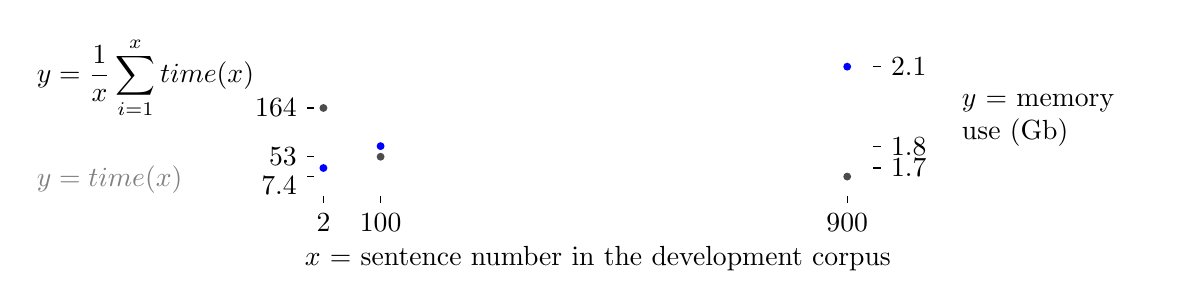
\begin{tikzpicture}
	%\draw[step=1,gray,very thin] (0,0) grid (10,3);
	%\draw[<->] (0,1.5) -- (0,0) -- (10,0);
	\node [anchor=east,text width=3.0cm] at (-0.5,1.3) {$\displaystyle y = \frac{1}{x}\sum_{i=1}^x time(x)$};
	\node [anchor=east,text width=2.5cm] at (-1,0) {\textcolor{gray}{$y = time(x)$}};
	\node [anchor=west,text width=2.5cm]  at (8,0.75) {$y$ = memory use (Gb)};
	\node at (3.5,-1.0) {$x$ = sentence number in the development corpus};
	\draw (0.0148148,-0.2) -- +(0.0,-0.1) node [anchor=north] {2};
	\draw (0.740741,-0.2) -- +(0.0,-0.1) node [anchor=north] {100};
	\draw (6.66667,-0.2) -- +(0.0,-0.1) node [anchor=north] {900};
	\draw[gray,thick] plot file {chap-algorithms/data-cache-by-sent};
	\draw[black,thick] plot file {chap-algorithms/data-cache-avg};
	\draw[blue,thick] plot file {chap-algorithms/data-cache-mem};
	
	\fill[blue] (0.0148148, 0.150011) circle (0.05);
	\fill[blue] (0.740741, 0.427965) circle (0.05);
	\fill[blue] (6.66667, 1.43709) circle (0.05);
	\draw (7.0,0.150011) -- +(0.1,0.0) node [anchor=west] {1.7};
	\draw (7.0,0.427965) -- +(0.1,0.0) node [anchor=west] {1.8};
	\draw (7.0,1.43709) -- +(0.1,0.0) node [anchor=west] {2.1};

	\fill[black!70] (0.0148148, 0.912278) circle (0.05);
	\fill[black!70] (0.740741, 0.293146) circle (0.05);
	\fill[black!70] (6.66667, 0.0412488) circle (0.05);
	\draw (-0.1,0.912278) -- +(-0.1,0.0) node[anchor=east] {164};
	\draw (-0.1,0.293146) -- +(-0.1,0.0) node[anchor=east] {53};
	\draw (-0.1,0.0412488) -- +(-0.1,0.0) node[anchor=east,text height=13pt] {7.4};
\end{tikzpicture}

	\end{center}
	\figpostamble
	\caption{Effect of caching on average and per-sentence lookup time and memory use.}
	\label{fig:caching-results}
\end{figure}

Finally, we observed that much of the gain from 
precomputation seemed to occur with very frequent patterns.
To test this, we ran experiments using precomputed collocations
and inverted indices for only the 100 most frequent patterns.
We found that the cost in memory use was reduced by nearly half.
In trade, per-sentence query time increased by 67\%, but in
absolute terms the increase was less than a second.

\begin{table}
	\begin{tabular}{ccc}
		Number of frequent patterns & memory use & query time \\ \hline
		1000 & 2.1G & 0.97 \\
		100 & 1.1G & 1.62\\
	\end{tabular}
	\caption[Effect of precomputation on memory use and processing time]
	{Effect of precomputation on memory use and processing time.  Here we show the memory requirement of the entire system ({\em sans} language model), including all data structures on the training data.}
	\label{fig:memory-usage}
\end{table}



\subsection{Translation Quality Results}\label{sec:hiero-translation-results}

We measured translation accuracy the same way that
we did for our phrase-based system.  It is important to note that
the baseline hierarchical model uses a slightly different feature
set \citep{Chiang:2007:cl}.

\begin{itemize}
	\item A source-to-target phrase translation probability.
	\item A target-to-source phrase translation probability.
	\item A source-to-target lexical weight.
	\item A target-to-source lexical weight.
	\item A language model feature.
	\item A word count feature.
	\item A phrase count feature only for nonlexicalized rules (i.e. a rule containing no terminal symbols).
	\item A phrase count feature for lexicalized rules.
\end{itemize}

\noindent We did not use any special translation
modules for numbers, dates, names, and bylines.  Therefore,
we leave out the associated features used by \citet{Chiang:2007:cl}.

We again study the effect of sampling and the effect of 
losing the baseline target-to-source feature, and we again noticed
during development that the phrase count features did not
correlate with accuracy.  Therefore, we tested the effect of
leaving out these features.  The results on a baseline system
using direct representation are given in Table~\ref{table:hiero-baselines}.
None of the differences were statistically significant.  This
confirms that neither the the target-to-source translation
probability nor the phrase penalties are essential to the system.
Therefore, we run the remaining experiments without the 
phrase penalties.  By design, we must leave out the target-to-source
probability.

\begin{table}
	\begin{center}
	\begin{tabular}{lc}
		Configuration & BLEU \\ \hline
		baseline with standard eight features & 30.7 \\
		baseline without target-to-source translation feature & 30.5 \\
		baseline without target-to-source translation or phrase count features & 30.6 \\
		baseline without phrase count feature & 30.7 \\
	\end{tabular}
	\end{center}
	\caption{Baseline system results compared with systems missing one or more features.}
	\label{table:hiero-baselines}
\end{table}

Results for translation by pattern matching are given in 
Table~\ref{table:hiero-sampling}.  As with the phrase-based
system, we find that we can match our baseline system 
results with a sampling size between two and three hundred.
Minor improvements obtained with larger sample sizes were
not statistically significant.  For results reported in 
the remainder of this dissertation, we use a sample
size of 300.

\begin{table}
	\begin{center}
		\begin{tabular}{ccc}
	sample size & time & BLEU \\ \hline
	0 & 0.97 & -- \\
	10   & 1.19 & 27.8 \\
	25   & 1.41 & 29.6 \\
	50   & 1.66 & 30.1 \\
	100  & 2.04 & 30.4 \\
	200  & 2.70 & 30.8 \\
	300  & 3.27 & 30.9 \\
	400  & 3.76 & 30.8 \\
	500  & 4.25 & 31.2 \\
	1000 & 6.25 & 30.9 \\
\end{tabular}
	\end{center}
	\caption{Effect of different sampling sizes on per-sentence times for query, extraction, and scoring and translation accuracy.}
	\label{table:hiero-sampling}
\end{table}

As before, we find that extraction adds significant time
to the overall speed.  This is partly an artifact of 
our implementation, which scans all alignment links for a sentence
in order to compute the target span and its reflection.  To
improve efficiency, we could design an alignment data structure
that only stores the indices of the rightmost and leftmost aligned words for 
each source and target word.  This representation would enable
random access, since the number of tokens would be equal to
the size of the text, and thus its indexes would correspond.
However, we are able to replicate the results of a direct representation
using quite a small sample size.

\section{Conclusion}\label{sec:algorithms-conclusions}

The innovations described in this chapter solve a computationally
challenging puzzle of efficient pattern matching with discontiguous
phrases.  We believe this is intrinsically
interesting from an algorithmic perspective.
However, our main interest is that it enables us to apply translation
by pattern matching to practically any MT model, provided 
that model-specific rule extraction algorithms are developed.  
In the next chapter, we will show that our algorithms facilitate
streamlined experimentation with hierarchical models, and that
we can improve hierarchical phrase-based translation in a
way that is not practical with a direct representation.



